\documentclass[]{article}
\usepackage{lmodern}
\usepackage{amssymb,amsmath}
\usepackage{ifxetex,ifluatex}
\usepackage{fixltx2e} % provides \textsubscript
\ifnum 0\ifxetex 1\fi\ifluatex 1\fi=0 % if pdftex
  \usepackage[T1]{fontenc}
  \usepackage[utf8]{inputenc}
\else % if luatex or xelatex
  \ifxetex
    \usepackage{mathspec}
  \else
    \usepackage{fontspec}
  \fi
  \defaultfontfeatures{Ligatures=TeX,Scale=MatchLowercase}
\fi
% use upquote if available, for straight quotes in verbatim environments
\IfFileExists{upquote.sty}{\usepackage{upquote}}{}
% use microtype if available
\IfFileExists{microtype.sty}{%
\usepackage[]{microtype}
\UseMicrotypeSet[protrusion]{basicmath} % disable protrusion for tt fonts
}{}
\PassOptionsToPackage{hyphens}{url} % url is loaded by hyperref
\usepackage[unicode=true]{hyperref}
\hypersetup{
            pdftitle={Machine Learning 2 Project},
            pdfauthor={Silke Meiner, Rafaela Neff},
            pdfborder={0 0 0},
            breaklinks=true}
\urlstyle{same}  % don't use monospace font for urls
\usepackage[margin=1in]{geometry}
\usepackage{natbib}
\bibliographystyle{plainnat}
\usepackage{graphicx,grffile}
\makeatletter
\def\maxwidth{\ifdim\Gin@nat@width>\linewidth\linewidth\else\Gin@nat@width\fi}
\def\maxheight{\ifdim\Gin@nat@height>\textheight\textheight\else\Gin@nat@height\fi}
\makeatother
% Scale images if necessary, so that they will not overflow the page
% margins by default, and it is still possible to overwrite the defaults
% using explicit options in \includegraphics[width, height, ...]{}
\setkeys{Gin}{width=\maxwidth,height=\maxheight,keepaspectratio}
\IfFileExists{parskip.sty}{%
\usepackage{parskip}
}{% else
\setlength{\parindent}{0pt}
\setlength{\parskip}{6pt plus 2pt minus 1pt}
}
\setlength{\emergencystretch}{3em}  % prevent overfull lines
\providecommand{\tightlist}{%
  \setlength{\itemsep}{0pt}\setlength{\parskip}{0pt}}
\setcounter{secnumdepth}{0}
% Redefines (sub)paragraphs to behave more like sections
\ifx\paragraph\undefined\else
\let\oldparagraph\paragraph
\renewcommand{\paragraph}[1]{\oldparagraph{#1}\mbox{}}
\fi
\ifx\subparagraph\undefined\else
\let\oldsubparagraph\subparagraph
\renewcommand{\subparagraph}[1]{\oldsubparagraph{#1}\mbox{}}
\fi

% set default figure placement to htbp
\makeatletter
\def\fps@figure{htbp}
\makeatother


\title{Machine Learning 2 Project}
\author{Silke Meiner, Rafaela Neff}
\date{20 3 2021}

\begin{document}
\maketitle

{
\setcounter{tocdepth}{2}
\tableofcontents
}
\section{Abstract}\label{abstract}

We present and compare machine learnt classification algorithms for
diagnosing breast tumor cells as benign or malignant. The algorithms
were trained on tabular data consisting of features extracted from
microscopic images of fine-needle aspirates / biopsies.

We get reasonably good results from Logistic regression and were able to
improve these results through single and multi-layer neural networks.
The final neural network with an accuracy of 98\%, sensitivity of 1 and
specificity 1 is being audited at the German Gesundheitsministerium to
become a state approved diagnostic tool.

The layout of this paper follows the CRISP-DM model.

\section{Business Understanding}\label{business-understanding}

Breast cancer is the most common cancer for women and ranks highest for
cancer-related deaths in women in Germany: In 2016 there were 68,950
women and 710 men suffering from Breast Cancer (ICD-10 C50). In 2020
18,570 women and 1 men have died of breast cancer. The situation is
similar in many other countries.

Tumors can build in the human body as some cells grow more than they
normally should. If this growth is not limiting itself and destroys body
tissue and hinders body functions the tumor is labeled malignant and
called cancer.

Tumors are classified in a binary fashion as either malignant or benign.
Their difference in microscopic imagery are shown in figure
\ref{fig:normal-vs-cancer}. A typical first step when diagnosing a tumor
is to do a fine needle aspirate (FNA) of a breast mass and looking at
the cells through a microscope, describing characteristics of the cell
nuclei. Further treatment differs according to the tumor diagnosis as
benign or malignant.

\begin{figure}
    \centering
    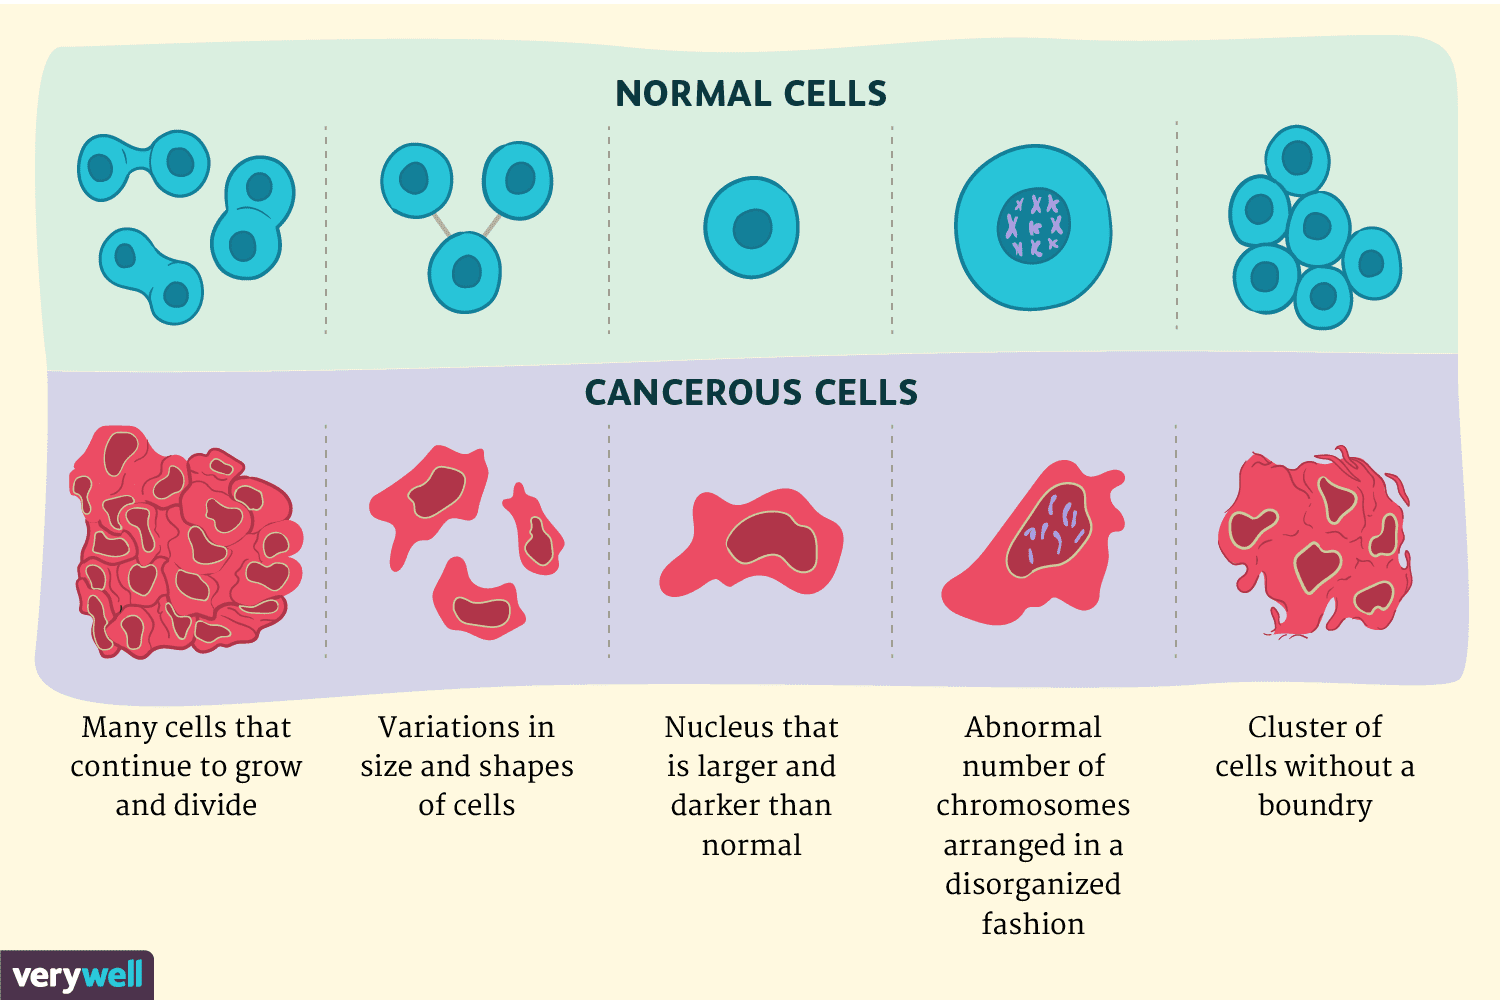
\includegraphics[width=0.8\textwidth]{images/normal-vs-cancerous-cells.png}
    \caption{benign / normal and malignant / cancerous  cells}
    \label{fig:normal-vs-cancer}
\end{figure}

In medical diagnostics, based on human or artificial intelligence,
correctness is very important. It is described in terms of sentitivity
and specificity. Both are measured in percentage. Sensitivity is the
true positive rate, the rate at which malignant tumors are correctly
identified. Specificity is the true negative rate, the rate at which a
patients concerns can correctly be relieved.

Sources :

\begin{itemize}
\item
  \cite{rki}
\item
  \cite{malignant-and-benign}
\item
  \cite{cancer-cells-vs-normal}
\end{itemize}

\section{Data Sources and Data
Understanding}\label{data-sources-and-data-understanding}

The data for this project was collected in 1995 by the University of
Wisconsin and made available to us through Prof.~Dr.~Nick Street of the
University of Iowa.

The data can be downloaded from the University of California, Irvine,
\url{https://archive.ics.uci.edu/ml/datasets/Breast+Cancer+Wisconsin+\%28Diagnostic\%29}

\subsection{Data Understanding}\label{data-understanding}

Our data set is mid sized with 569 observations for 30 numeric feature
variables. Each observation has an additional binary diagnosis as benign
or malignant. The data set is slightly unbalanced with 357 (63\%) benign
and 212 (37\%) malignant cases. We made malignant the positive class.

\begin{figure}
    \centering
    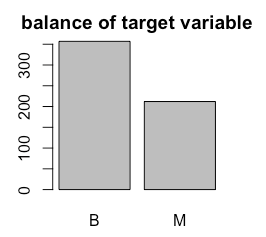
\includegraphics[width=0.4\textwidth]{images/binary-classification.png}
    \caption{classes in the binary classification task, B: benign, M: malignant / cancerous}
    \label{fig:bin_class}
\end{figure}

In figure \ref{fig:cor-1} we present the correlation of features and
find some features / predictor variables highly correlated.

\begin{figure}
    \centering
    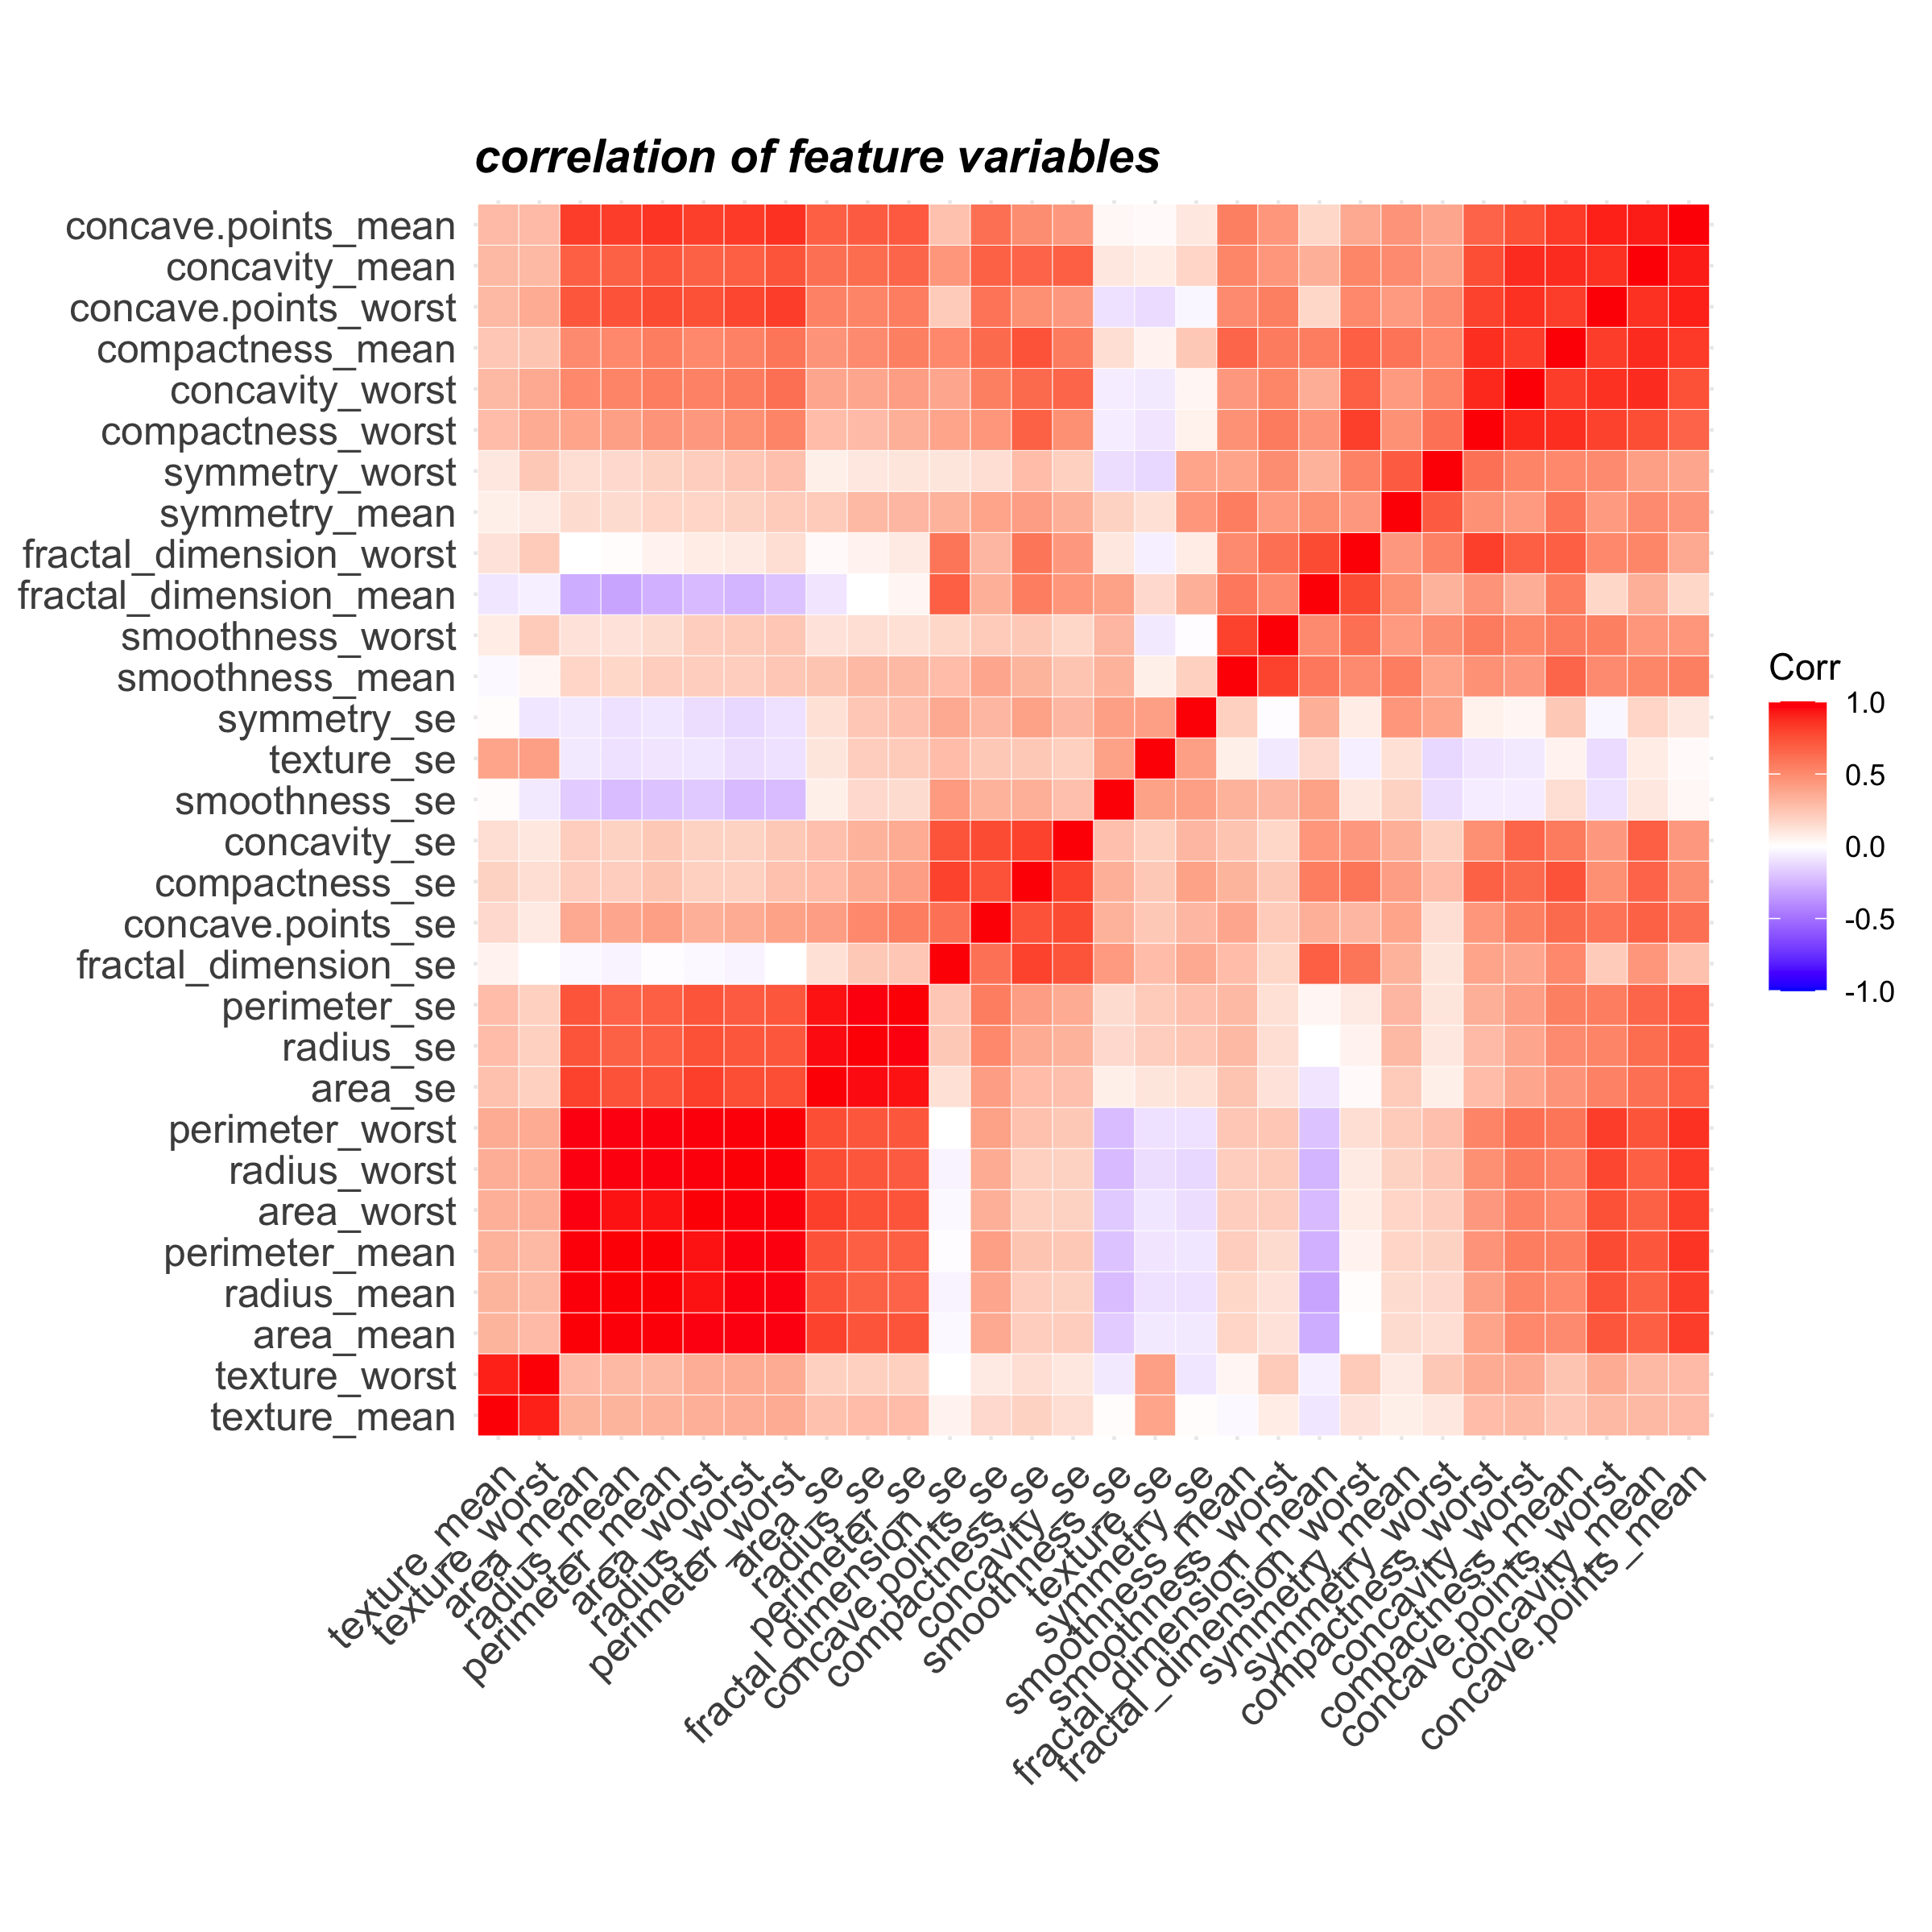
\includegraphics[width=0.8\textwidth]{images/correlation-features.png}
    \caption{correlation of feature variables}
    \label{fig:cor-1}
\end{figure}

We point out three groups of correlated features:

The group of most highly (and positively) correlated features correspond
to the description of malignant / cancerous cells given in
\ref{fig:normal-vs-cancer}: They describe cells wit a large and
irregular perimeter, radius and area:

\begin{itemize}
\tightlist
\item
  perimeter\_mean, perimeter\_worst
\item
  radius\_mean, radius\_worst
\item
  area\_mean, area\_worst
\end{itemize}

The second most highly (and positively) correlated group of features are
the standard errors for the cells perimeter, radius and area, underlying
the group of most highly correlated features.

\begin{itemize}
\tightlist
\item
  perimeter\_se
\item
  radius\_se
\item
  area\_se
\end{itemize}

A third group of high to mild positive correlation is for features
related to concavity and compactness.

\begin{itemize}
\tightlist
\item
  concave.points\_mean, concave.points\_worst
\item
  concavity\_mean, concavity\_worst
\item
  compactness\_mean, compactness\_worst
\end{itemize}

In figure \ref{fig:normal-vs-cancer} convexity is a feature in the
benign / normal cells. Its opposite, concavity, can easily be associated
with the malignant / cancerous cells.

When there is (positive) correlation of feature variables with the
target variable, it is most prominent for features from the first and
third group of correlated features. Positive correlation of target and
features is maximal for concave.points\_worst with a value of 0.794.

\textless{}\textless{}\textless{}\textless{}\textless{}\textless{}\textless{}
HEAD \#\# Data Visualisation, looped back after first modeling =======
In figure \ref{fig:densities} we present two density plots of our
features. Both features have a high (positive) correlation to the
target. Distributions are well distinguishable for the two classes which
is in advantage for the classification task.

\begin{figure}
    \centering
    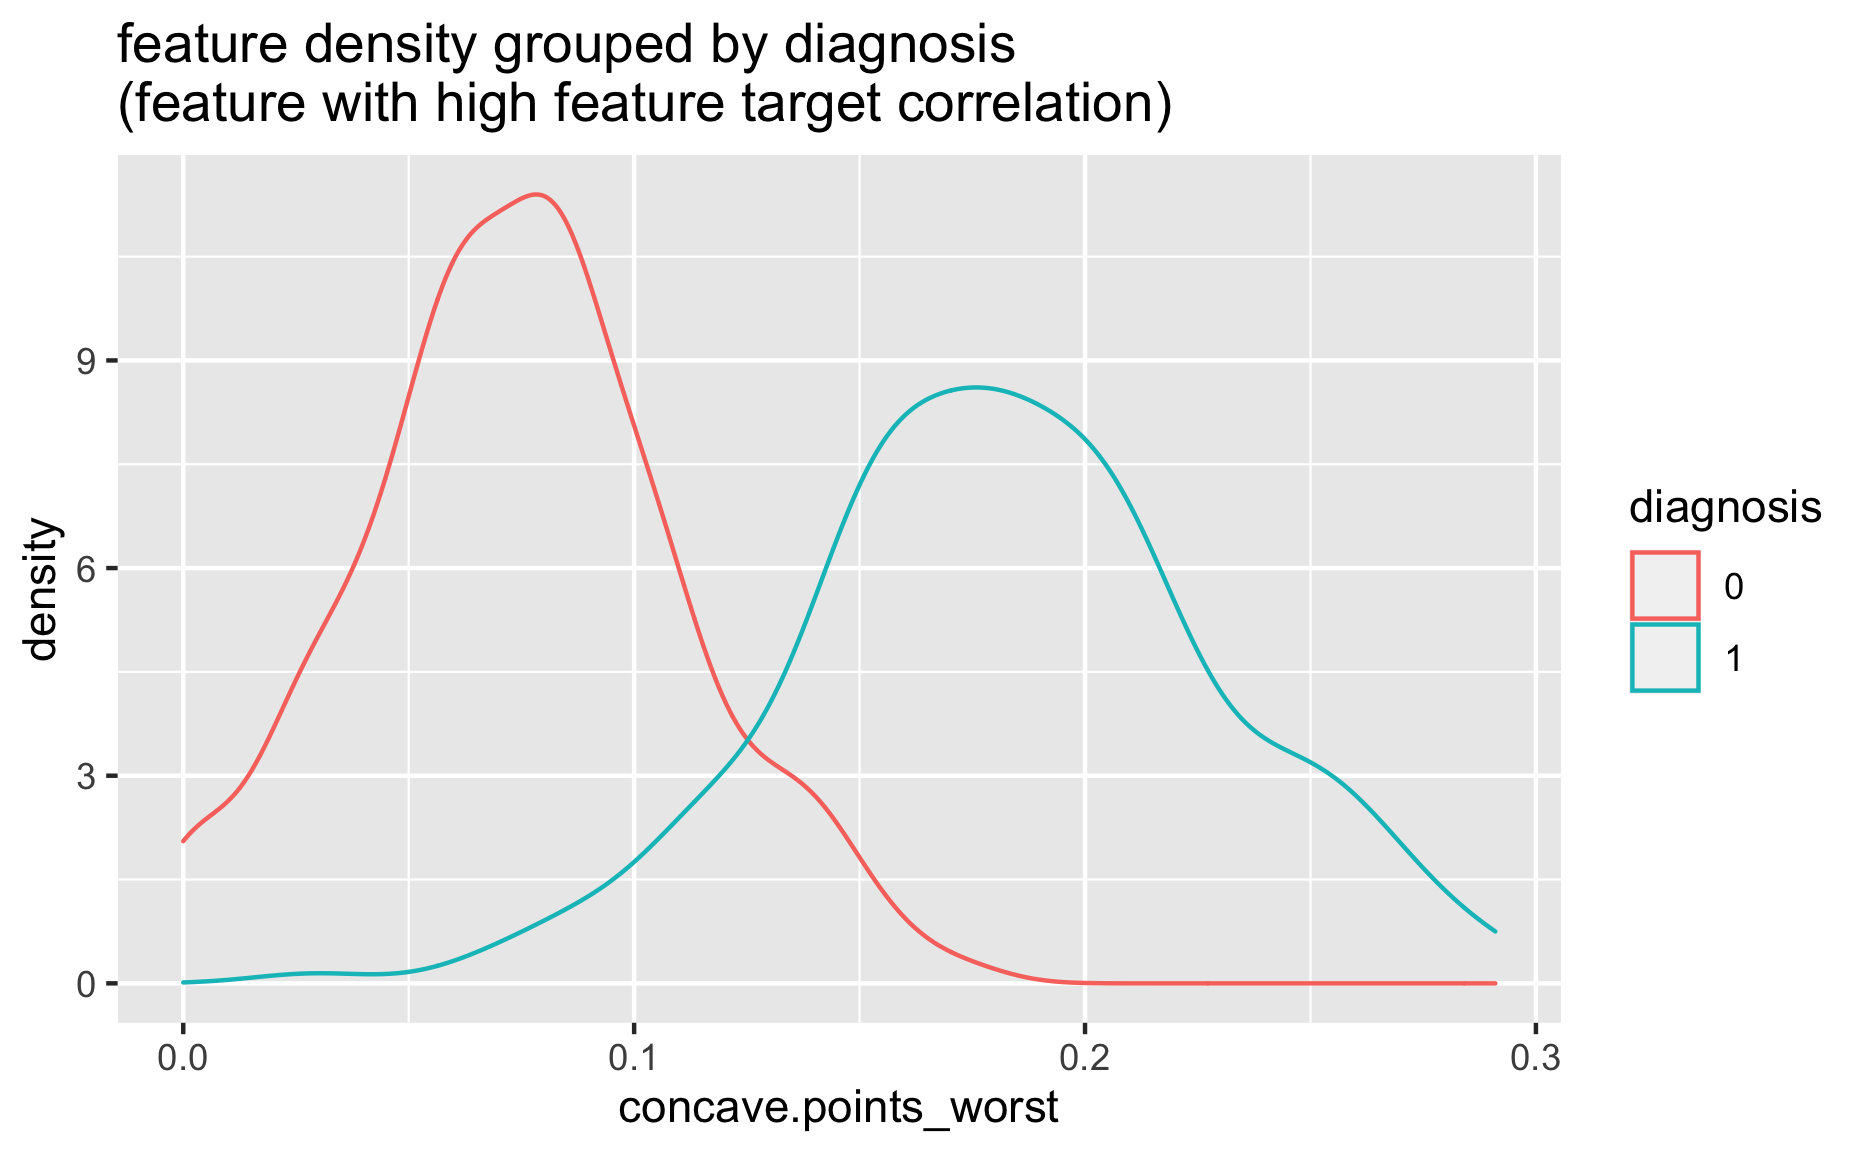
\includegraphics[width=0.45\textwidth]{images/density2.png}
    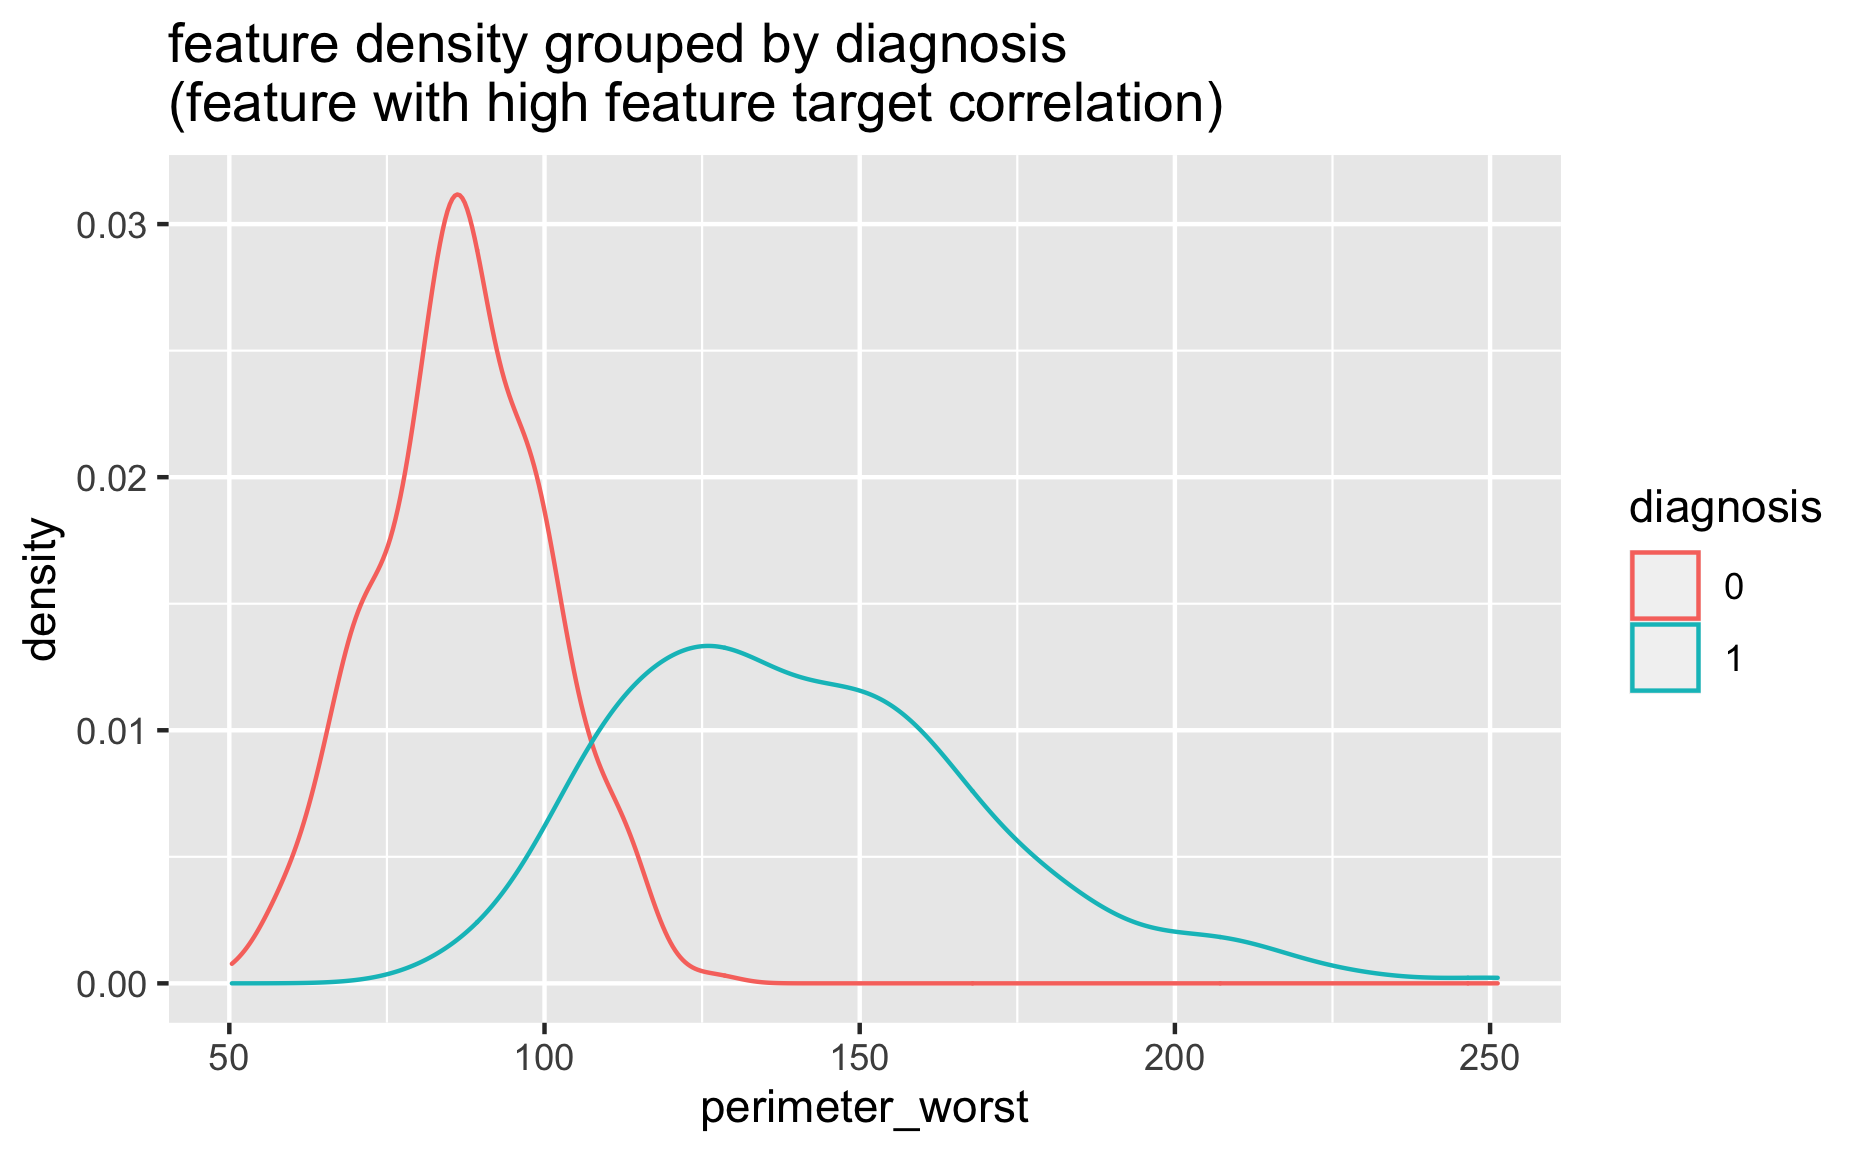
\includegraphics[width=0.45\textwidth]{images/density3.png}
    \caption{Density plots for two exemplary features}
    \label{fig:densities}
\end{figure}

For more density plots, please see our data-understanding.Rmd notebook.

The features in this data set seem hand crafted and contain expert
domain knowledge.

\subsection{Data Visualisation, looped back after first
modelling}\label{data-visualisation-looped-back-after-first-modelling}

\begin{quote}
\begin{quote}
\begin{quote}
\begin{quote}
\begin{quote}
\begin{quote}
\begin{quote}
4619ece6a083a2817838dfd53a5af13f72ff76ff
\end{quote}
\end{quote}
\end{quote}
\end{quote}
\end{quote}
\end{quote}
\end{quote}

This visualisation of our data by application of PCA was developed after
a first loop in the CRISP model. In sequential reading this serves as a
general visualisation now and will also be relevant later on.

\begin{figure}
    \centering
    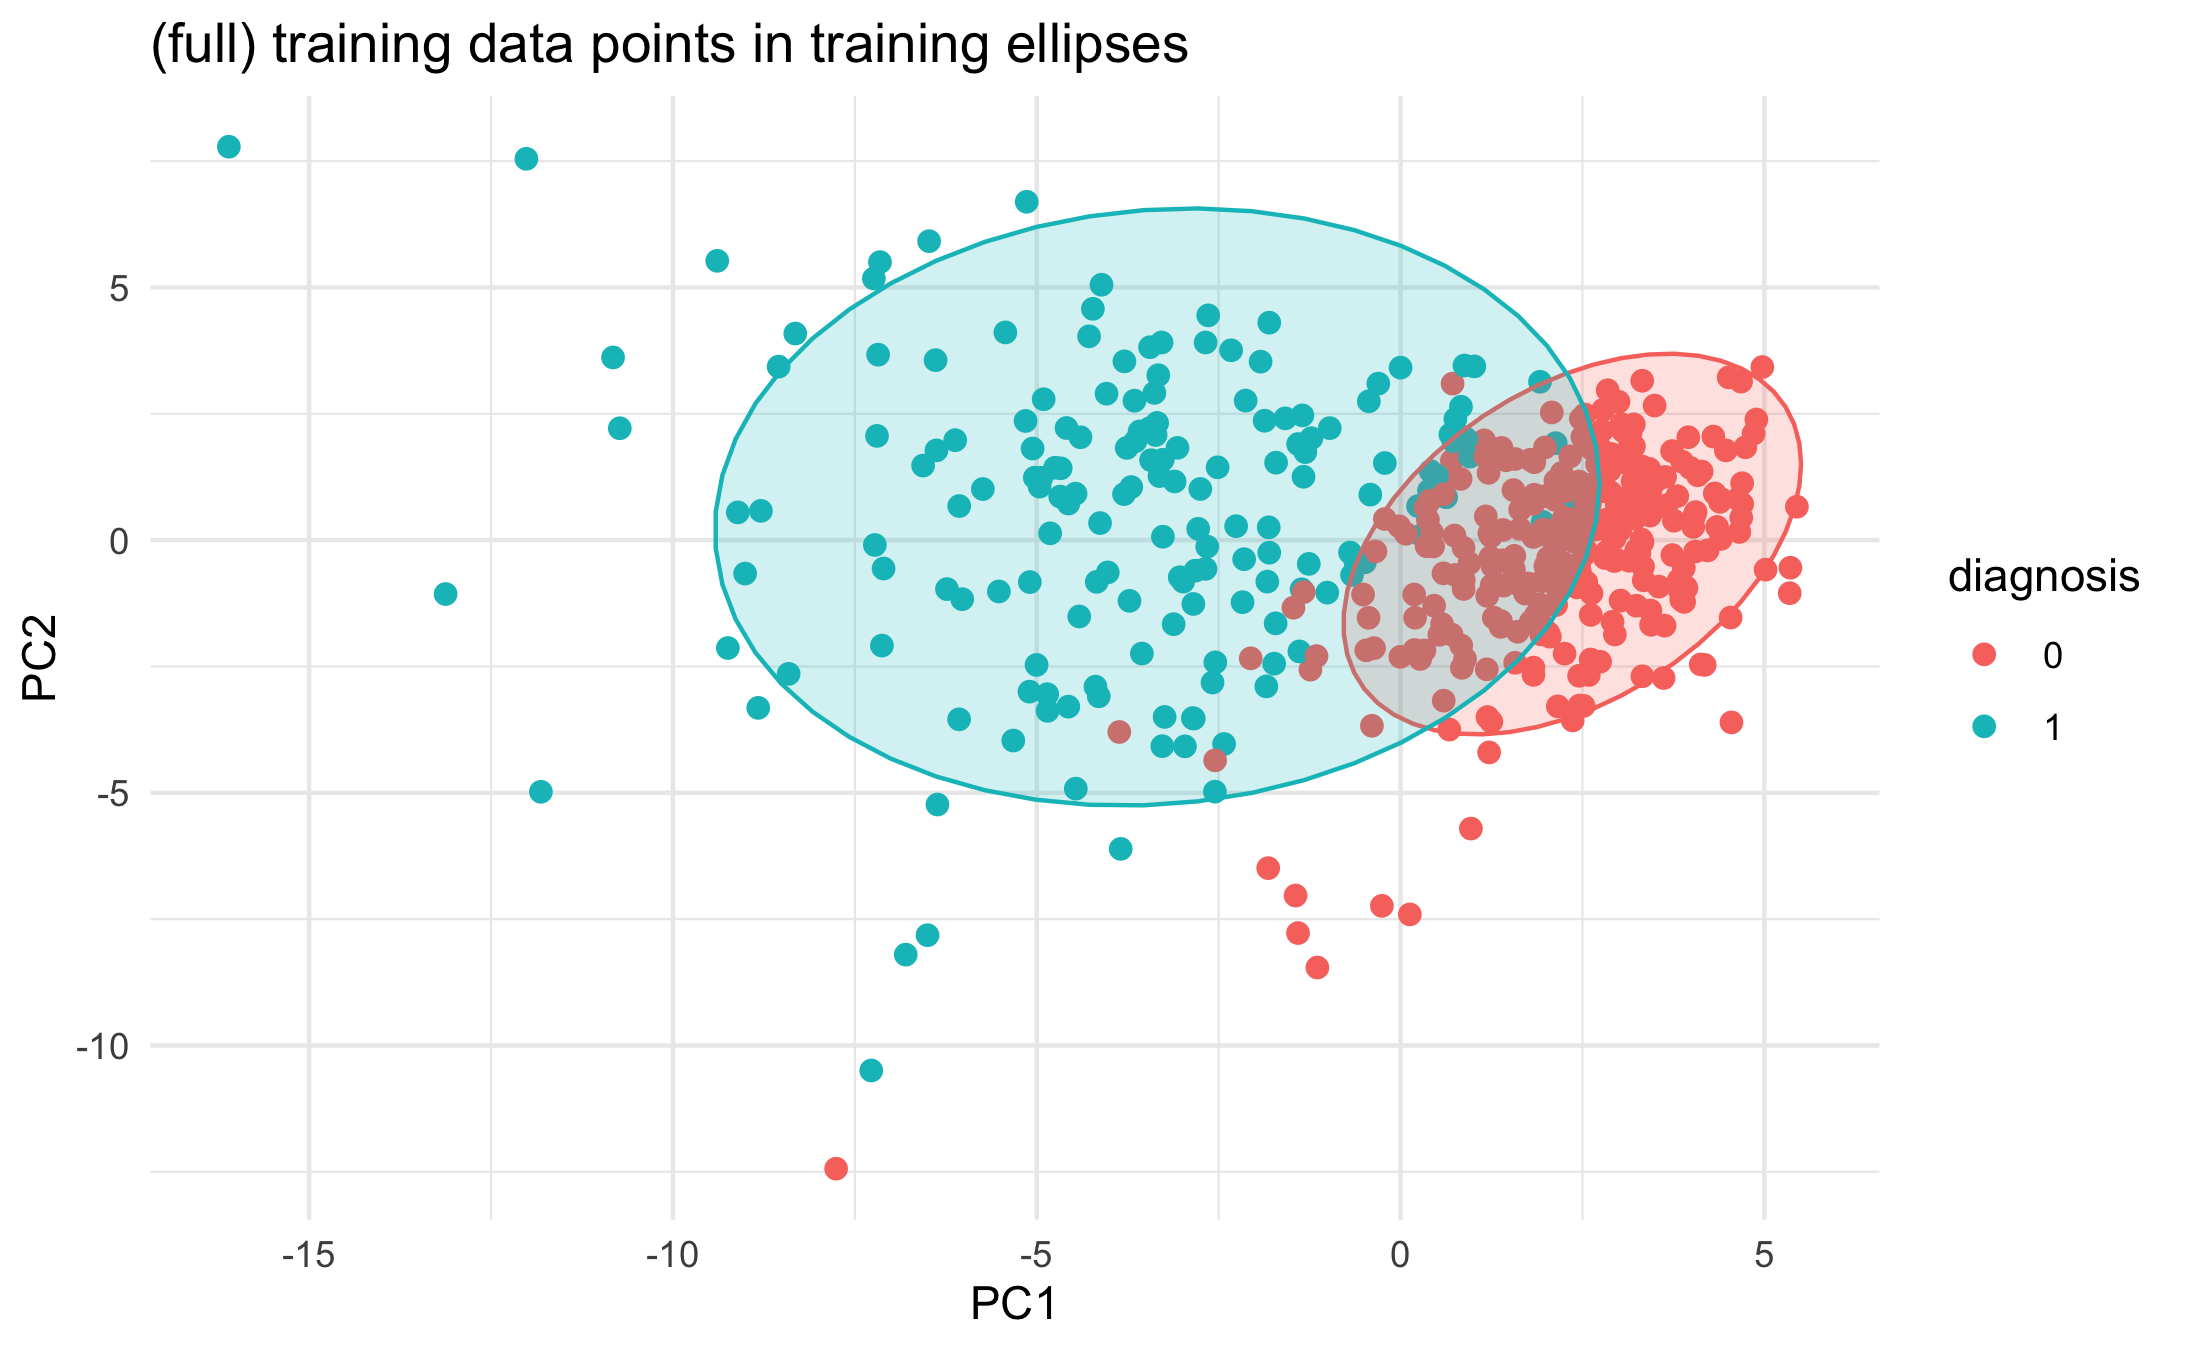
\includegraphics[width=0.8\textwidth]{images/A-training-full-PCA.png}
    \caption{PCA for the full training data}
    \label{fig:A-training-full-PCA}
\end{figure}

\section{Data Preparation}\label{data-preparation}

Since there were no missing data in our set we did not impute anything.
Data was used as delivered.

Data was separated into training and test sets, each with a separate
file. The data was split 80/20 and with stratification wrt to the
diagnosis.

For further details, please look into our notebook data-preparation.Rmd
.

\section{Modeling}\label{modeling}

To solve the classification task we applied two machine learning
methods: Logistic regression and neural networks.

In classification tasks we generally have predictor variables and a
target variable. In binary classification the target variable can take
one of two distinct values, interpreted as the two classes on option.

The methodological similarities of both machine learning models are in
the training and evaluation of the model. The training requires a
training set of observed data points including the true values of the
target variable. For evaluation a test set of observed data points
including the true values of the target variable is required. Training
and test set need to be disjoint. On the test set the algorithm predicts
classes for the data points and predictions are compared with the
targets. Counting correct and not correct classifications and setting
them in relation results in accuracy, sensitivity and specificity as
measures of success.

\subsection{Logistic Regression}\label{logistic-regression}

\subsubsection{Mathematical Background}\label{mathematical-background}

Given: Some numeric data, in tabular form of \(n\) rows and \(p+1\)
variables. \(p\) variables are predictors and the remaining variable is
the target. The target takes one of two values, interpreted as two
classes, with one class defined as the positive class.

Desired: The class the data point belongs to with a probability
distribution over the two classes (stating the probabilities that the
data point belongs to each class). Alternatively, the following result
would be of equal value: if or if not the data point belongs to the
positive class and the associated probability (single value in
{[}0,1{]}).

Linear regression uses a linear combination of the variables to predict
another numeric target variable. logistic regression does linear
regression for the log-odds of the desired probabilities.

\[
\text{log-odds} = \beta_0 + \beta_1 x_1 + \dots + \beta_p x_p     
\]

The log-odds are transformed into (conditional) probabilities for the
positive class through the logistic function \[\sigma(.)\], also called
sigmoid.

\[
p(\bf{x}) = \sigma(\text{log-odds}) = \sigma(\beta_0 + \beta_1 x_1 + \dots + \beta_p x_p ) 
\]

with (
\bf{x}= ( x_1, \dots, x_p) \) , \( p(\bf{x}) = \mathbf{P}\left(\text{target = positive class} | \text{predictors } = \bf{x} \right) \) and  \( \sigma(a) = \frac{1}{1+e^{-a}} \).

If the probability for the positive class (
p(\bf{x}) \)  exceeds a threshold, the data point is classified as the positive class.

The performance of the model is determined by its coefficients / weights
( \beta ). Finding the best / suitable coefficients is done in training.
For logistic regression there are several training methods performed by
statistical software like R.

In the beginning of running a logistic regression we ran into a
`problem' hinting at perfect separation of classes in our data set. We
decided to ignore this and try to get the best possible results from
logistic regression. Another option would have been: change to support
vector machines which could directly exploit the separability in our
data.

Sources:

Log Regression (\cite{logreg})

for ignoring the problem of complete separation (\cite{ucla})

Finding coefficients for logistic regression: (\cite{newton})

\subsubsection{Modeling in R}\label{modeling-in-r}

First attempts to run a logistic regression are documented in
log-reg-01.Rmd and log-reg-02.Rmd in the github repository's code
folder. The following presentation is based on log-reg-03.Rmd and uses
the caret library in R.

We compared different preprocessing options for the logistic regression:

\begin{itemize}
\tightlist
\item
  no preprocessing
\item
  center and scaleing
\item
  min-max-normalization to the interval {[}0,1{]}
\item
  PCA (including center and scaling)
\end{itemize}

Using 10 fold cross validation which was repeated 50 times (with new and
different sepatation of the training data into 10 subsets / folds one of
which would be used for validation) we obtained the following plot
\ref{fig:pre-proc-options} for accuracies for the different prepocessing
options.

\begin{figure}
    \centering
    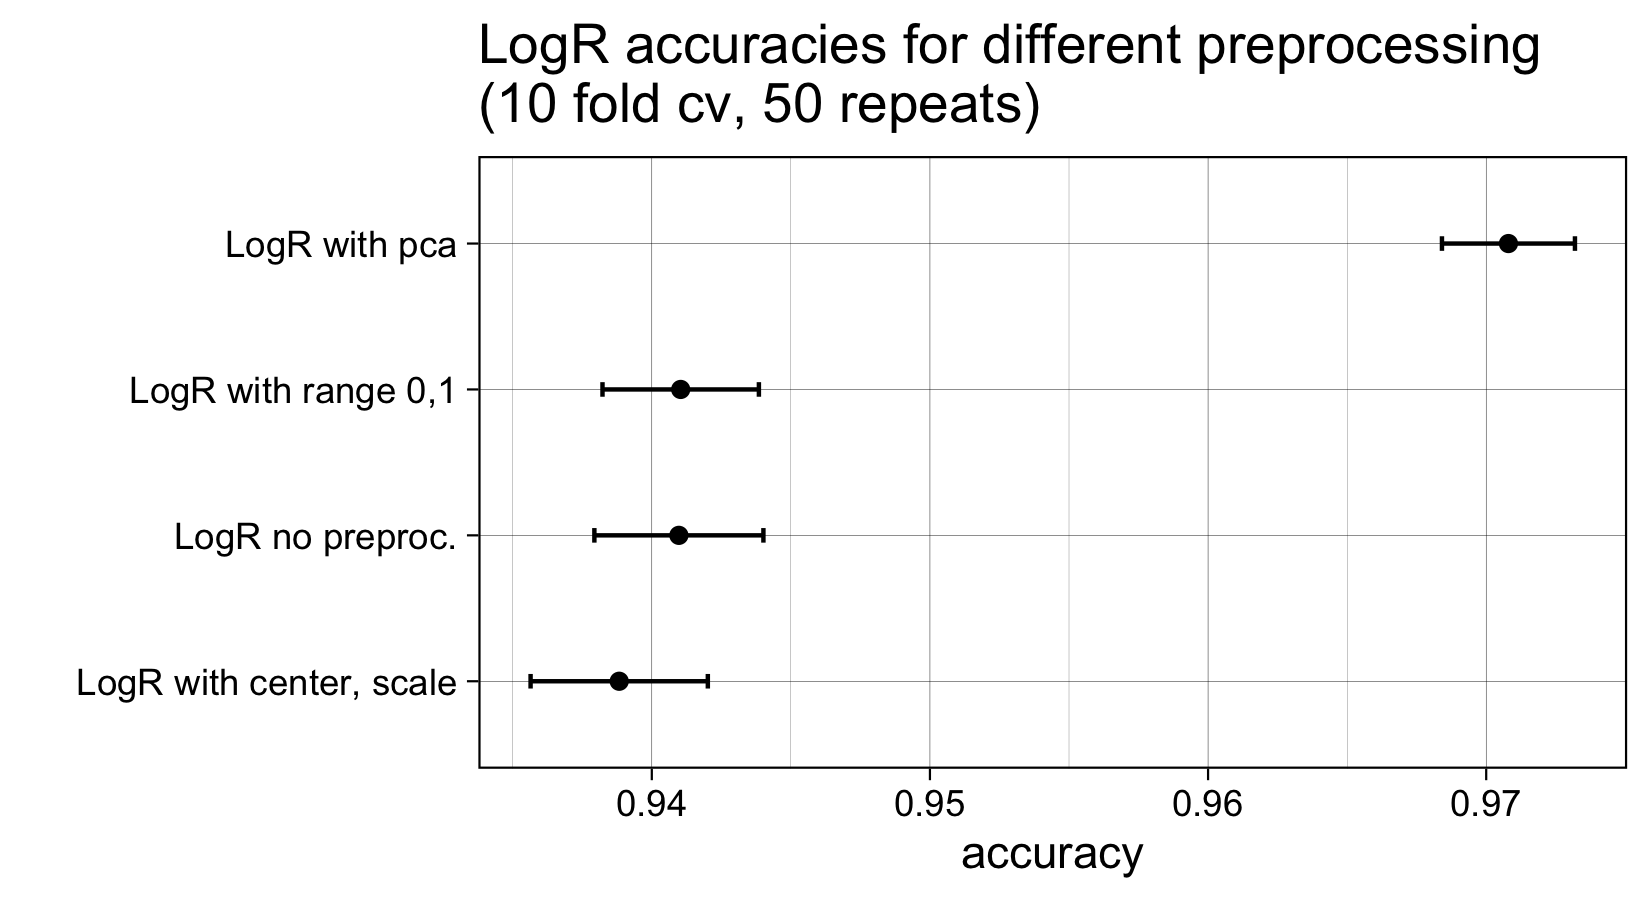
\includegraphics[width=0.8\textwidth]{images/preprocessing-options.png}
    \caption{accuracy for different pre-processing options}
    \label{fig:pre-proc-options}
\end{figure}

Principal component analysis (pca) shows by far the best result.

We also tested if removing correlated variables improves accuracy. This
can happen because removing highly correlated variables can be seen as
removing noise making it easier for the model to pick up relevant
structures in the data.

When looking at a group of highly correlated features all but one
features of the group were removed.

We tested removing features with 99\% correlation and with 97\%
correlation against the full feature set. We tested this for the
logistic regression with PCA pre-processing and for the logistic
regression with no pre-processing (cf figure
\ref{fig:feature-reduction-options}) arriving at the following results:

\begin{itemize}
\tightlist
\item
  Removing highly correlated variables seems to improve accuracy for the
  logistic regression algorithm on data that has not been pre-processed.
\item
  Removing highly correlated variables may or may not have an effect or
  a positive effect on accuracy for the logistic regression algorithm on
  data that has been pre-processed with pca.
\end{itemize}

\begin{figure}
    \centering
    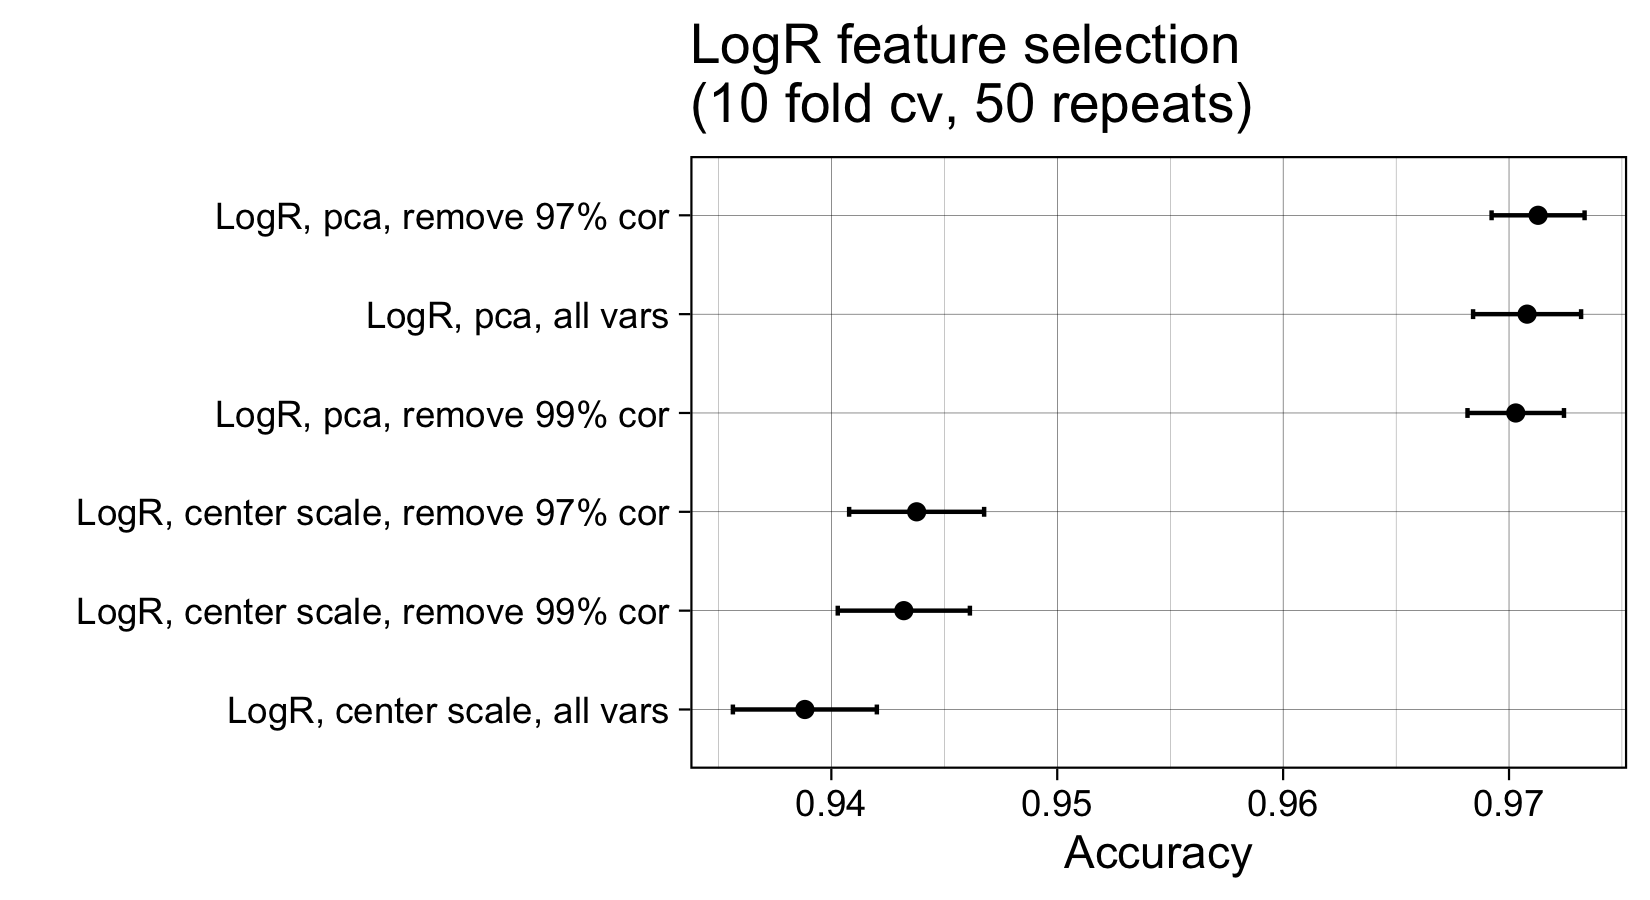
\includegraphics[width=0.8\textwidth]{images/feature-selection.png}
    \caption{accuracy for different reduced feature number}
    \label{fig:feature-reduction-options}
\end{figure}

This makes sense, as the PCA is a transformation of the data that
creates new variables that explain the data's variance, in descending
order. High correlation with previous principal components will not help
with explaining remaining variance.

As the over all best model we keep the best model from Logistic
Regression with a PCA as pre processing and the full set of variables
(mainly, we don't have a good enough reason to reduce features and throw
away information, especially when the PCA reduces information in a
reasonable, statistically approved way).

We arrived at our best model: logistic regression with PCA
pre-processing and the whole feature set. We then trained the model
again on the full training data. summary of the model is shown in figure
\ref{fig:logR-final-model}. The model did converge after 10 iterations,
some of the principal components are highly significant below 0.1\%.

\begin{figure}
    \centering
    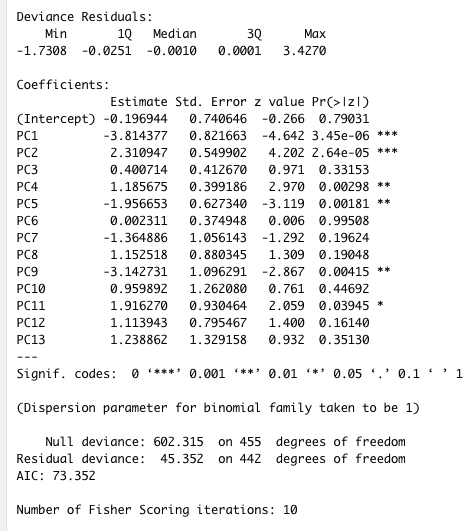
\includegraphics[width=0.6\textwidth]{images/logR_final_model.png}
    \caption{Final model for logistic regression}
    \label{fig:logR-final-model}
\end{figure}

From cross validation during training we obtained a mean accuracy of
96.5\% and mean sensitivity and specificity of 98.2\% (same for both).
In general, these are very acceptable results. In the medical domain we
should aim for better results, especially better sensitivity.

\subsection{Explainability}\label{explainability}

Logistic regression is a well explainable model. The ( \beta )
coefficients show the change in the log-odds for each feature variable
under the condition of all else equal. In our case with PCA
preprocessing we get coefficients that show the change in the log-odds
for each principal component. Since principal components are linear
combinations of the original features the all else equal condition will
not generally hold / be less realistic.

We state the results of the variable importance function (varImp) in R
caret in figure \ref{fig:logR_var_imp}

\begin{figure}
    \centering
    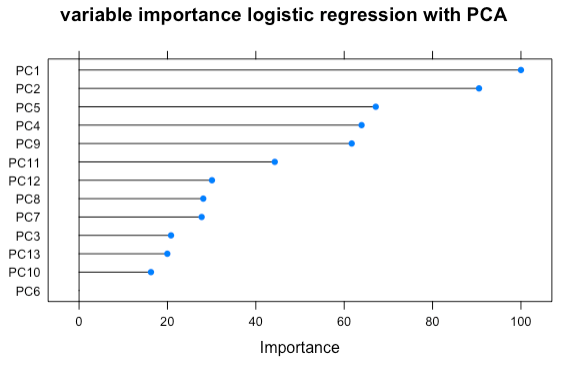
\includegraphics[width=0.6\textwidth]{images/logR_varImportance.png}
    \caption{variable importance for logistic regression with PCA}
    \label{fig:logR_var_imp}
\end{figure}

We try to apply black box interpretation models like variable shuffling.

\subsection{Artificial Neural
Networks}\label{artificial-neural-networks}

\subsubsection{Model overview}\label{model-overview}

Artificial Neural Networks are forecasting methods based on simple
mathematical models of the brain. They allow complex nonlinear
relationships between the response variable and its predictors.
(\cite{otexts})

\begin{figure}
    \centering
    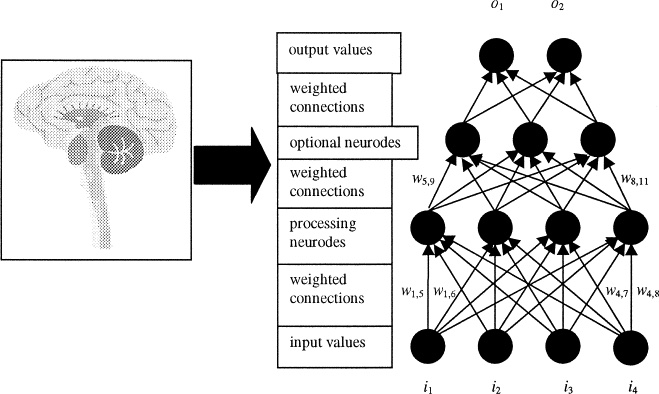
\includegraphics[width=0.8\textwidth]{images/ann.jpg}
    \caption{Sample artificial neural network architecture (not all weights are shown) - (\cite{ann})}
    \label{fig:ann}
\end{figure}

Connections between neurons are weighted to represent the connection
strength. It's the artificial pendant of the synapses in the brain.
Positive weights are used to excite neurons in the network and negative
weights are used to inhibit other neurons.

\textbf{Architecture}: Topology of the network

\textbf{Activities}: How do ANNs Neurons respond to one another to
produce a certain behavior.

\textbf{Learning Rule}: How should weights and connections change
regarding the input, output, and error-rate.

\textbf{Deep Neural Network}: Network with many hidden layers.

ANN structure can be described as its Architecture, Activities, and
Learning Rule.

\subsubsection{Implementation}\label{implementation}

We've implemented two different kinds of Neural Network. One wth R's
nnet-Package (\cite{nnet}) and one using the R-Package for h2o
(\cite{h2o}).

Nnet is supporting one hidden layer only and comes with poor
explainability. Since the results on the test-data were poor showing an
accuracy below 90\% we've choosen h2o over nnet and will evaluate
further on h2o throughout this report.

\subsection{Normalization}\label{normalization}

Depending on the implementation and the specific model different
standardization is used throughout this project in order to ensure that
all features have the same chance of importance fitting the model.

The nnet Implementation uses it's own user-defined-function (UDF)
standardizing via min-max-normalization using this formular: \[
\frac{x_i-\min(x_i)}{\max(x_i)-\min(x_i)}
\]

The h2o-Implementation uses the Standard Deviation implicitly,
standardazing via \[
\frac{x-mean}{stddev}
\]

\subsubsection{Proposed Model
architecture}\label{proposed-model-architecture}

We arrived at the selected Hyperparameters by performing a grid-search:

Activation function: Rectified Linear Input drop out ratio: 0.2 Hidden
layers : 3 sets each consisting of 3 layers Epoch: 500 Nfolds: 10

We've also tried Tanh and Maxout as activation function, with comparable
results.

Since we are training our model rather small dataset the classes were
balanced during training using the balance\_class parameter of the
h2o-package. Internal validation is done using 10-fold cross-validation
with stratified assignment.

We've chosen the model with the highest AUC-value which isn't 1. This
decision is based on preventing overfitting. The False-Negatives were
examined manually to get a grip on the real-world-value of our model.
What we are trying to prevent is our model telling that a person doesn't
have breast-cancer, when in fact he or she does.

Considering all this we did arrive at the following architecture:

\begin{figure}
    \centering
    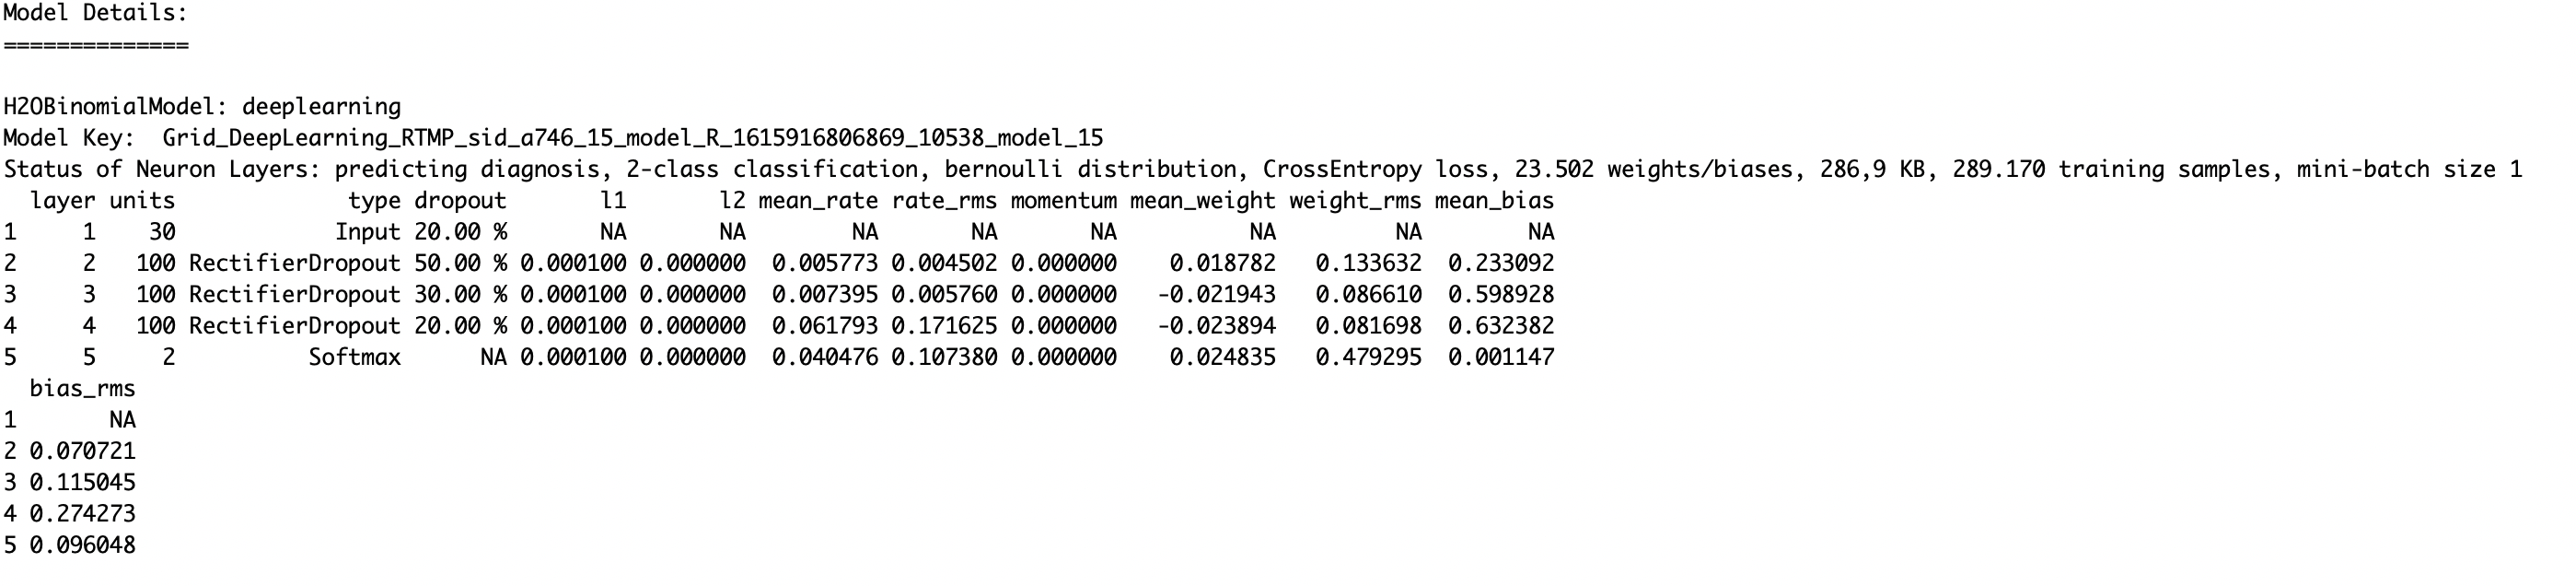
\includegraphics[width=1\textwidth]{images/model_details.png}
    \caption{Summary of the choosen Artificial Neural Network}
    \label{fig:model_details}
\end{figure}

\begin{figure}
    \centering
    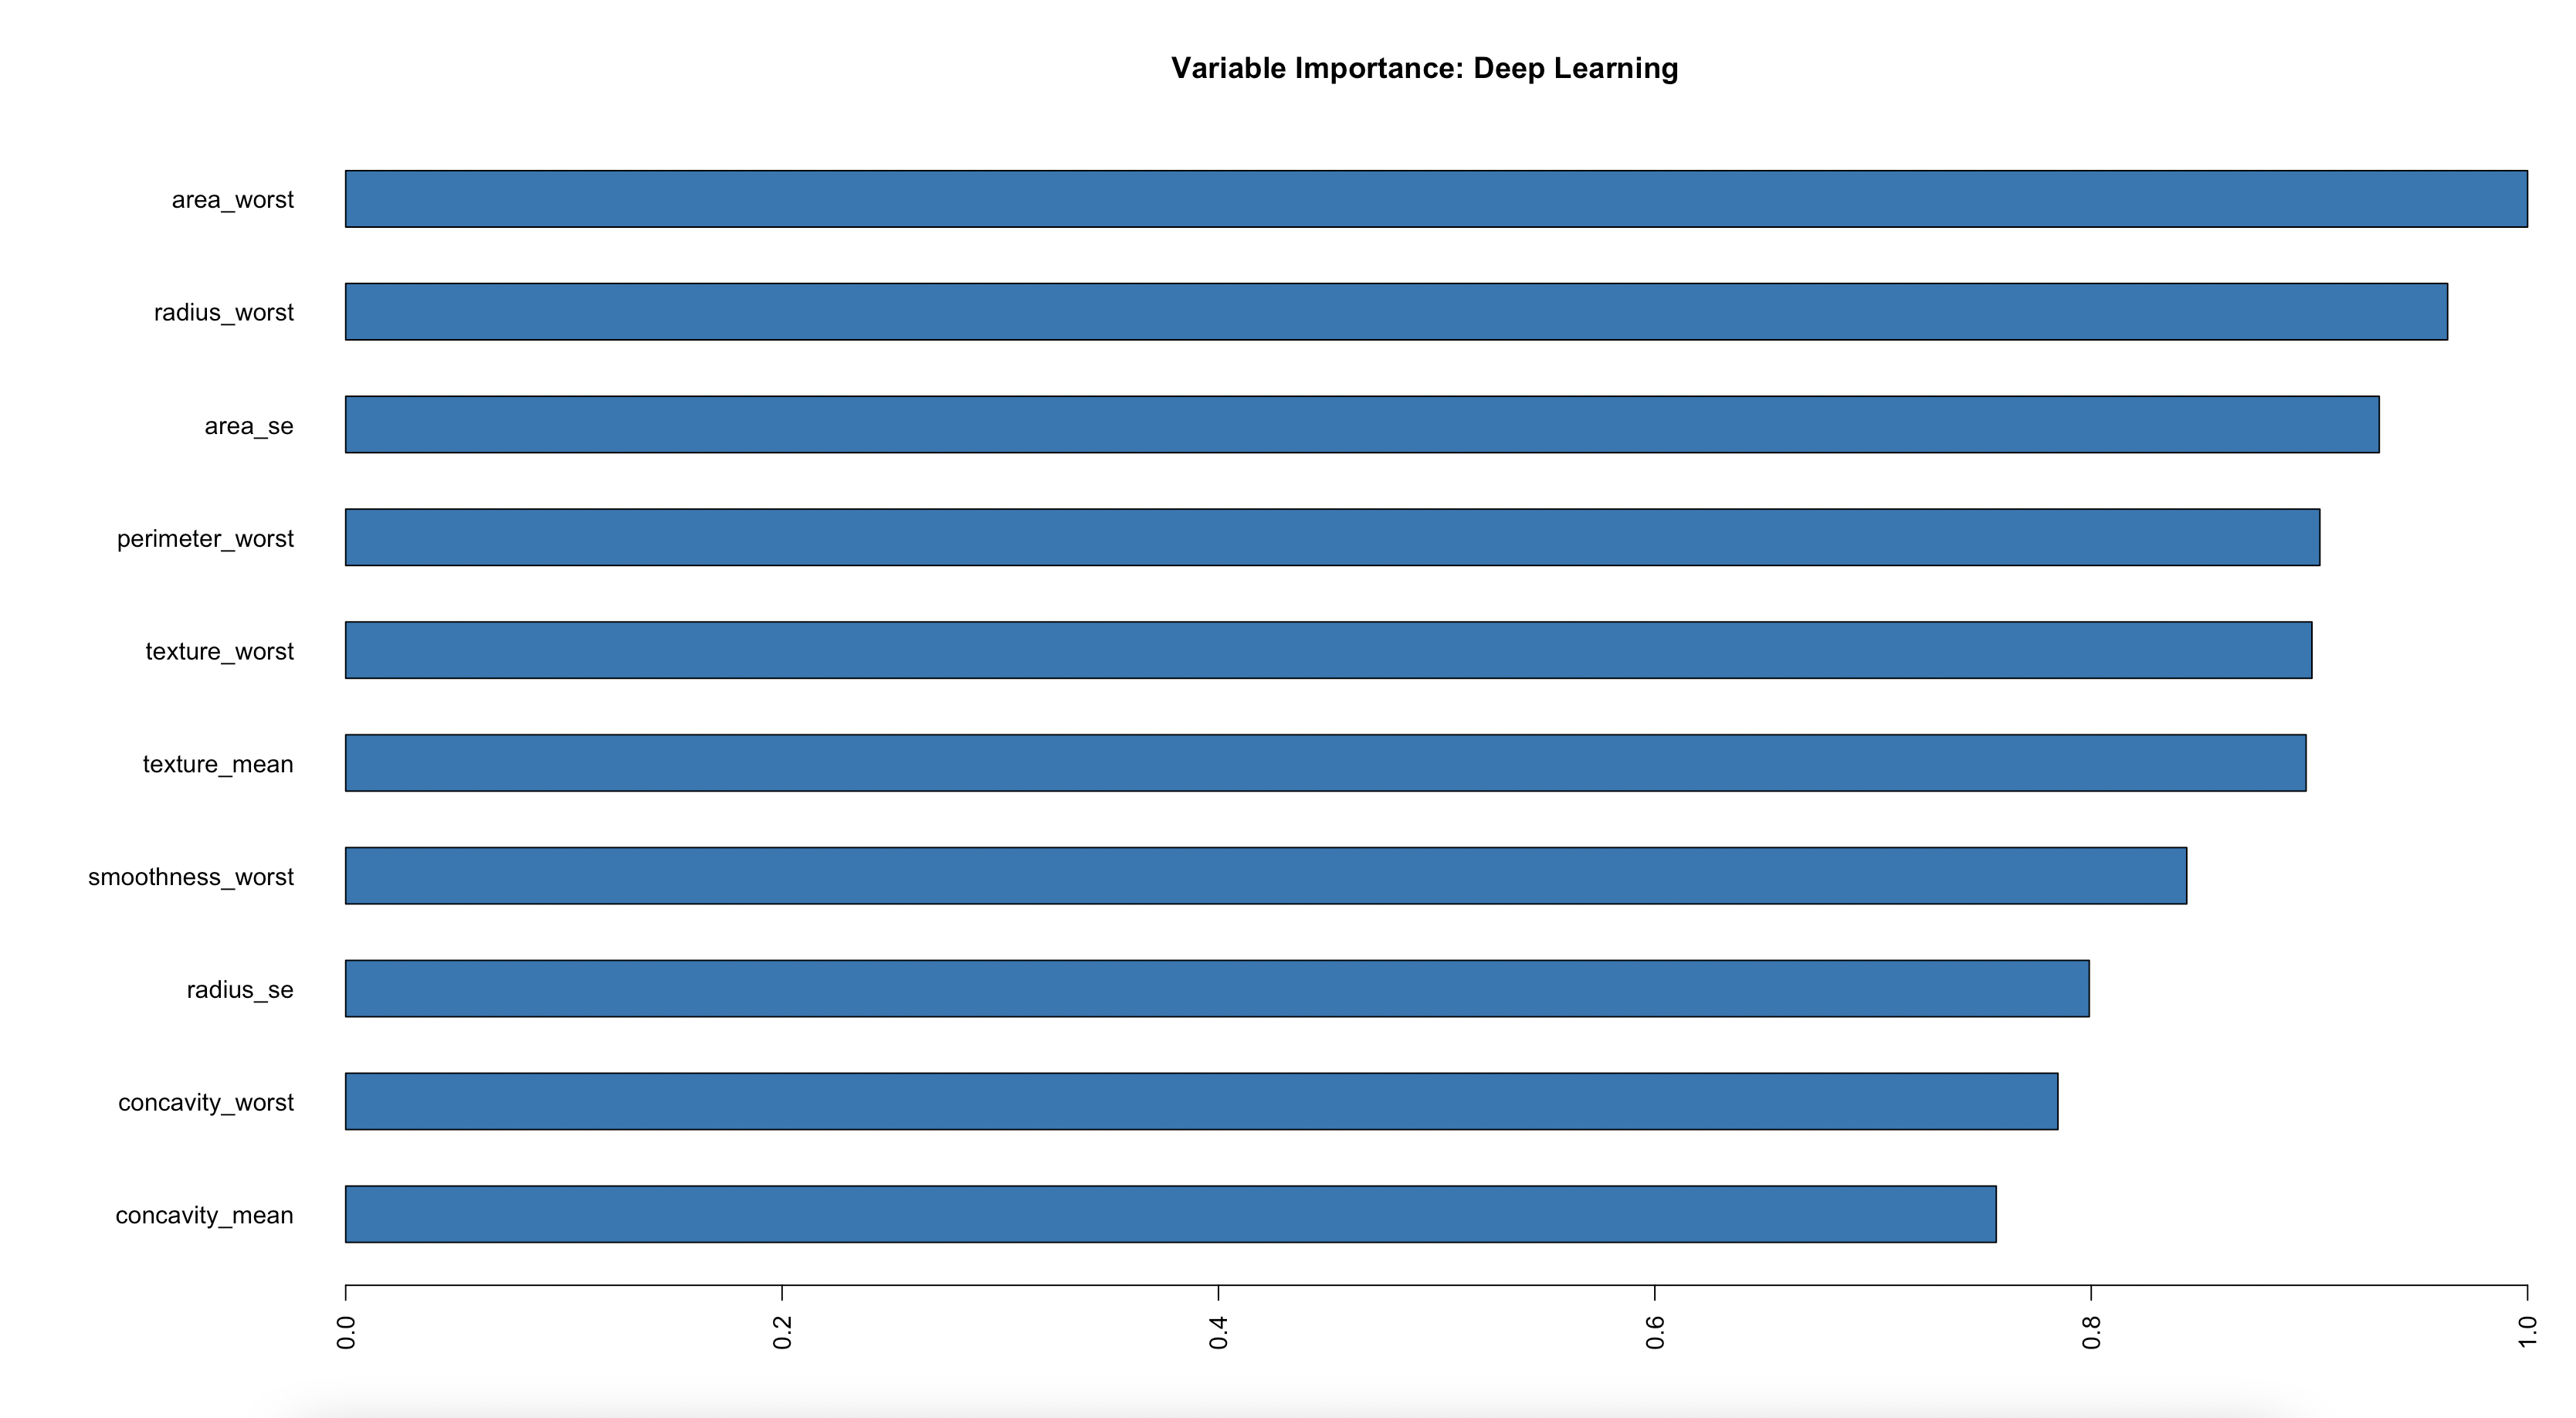
\includegraphics[width=0.8\textwidth]{images/variable_importance.png}
    \caption{Variable Importance of the choosen Artificial Neural Network}
    \label{fig:variable_importance}
\end{figure}

\subsubsection{Criteria}\label{criteria}

\paragraph{Explainibility}\label{explainibility}

We did choose the R-Package h2o over nnet for it's great explainability.

\paragraph{Expert Plots}\label{expert-plots}

A deeper understanding of a fittet model can be gained with a variety of
plots. For an ANN a Partial Dependence Plot or the Individual
Conditional Expectation Plot of a given column can be visualized.

\begin{figure}
    \centering
    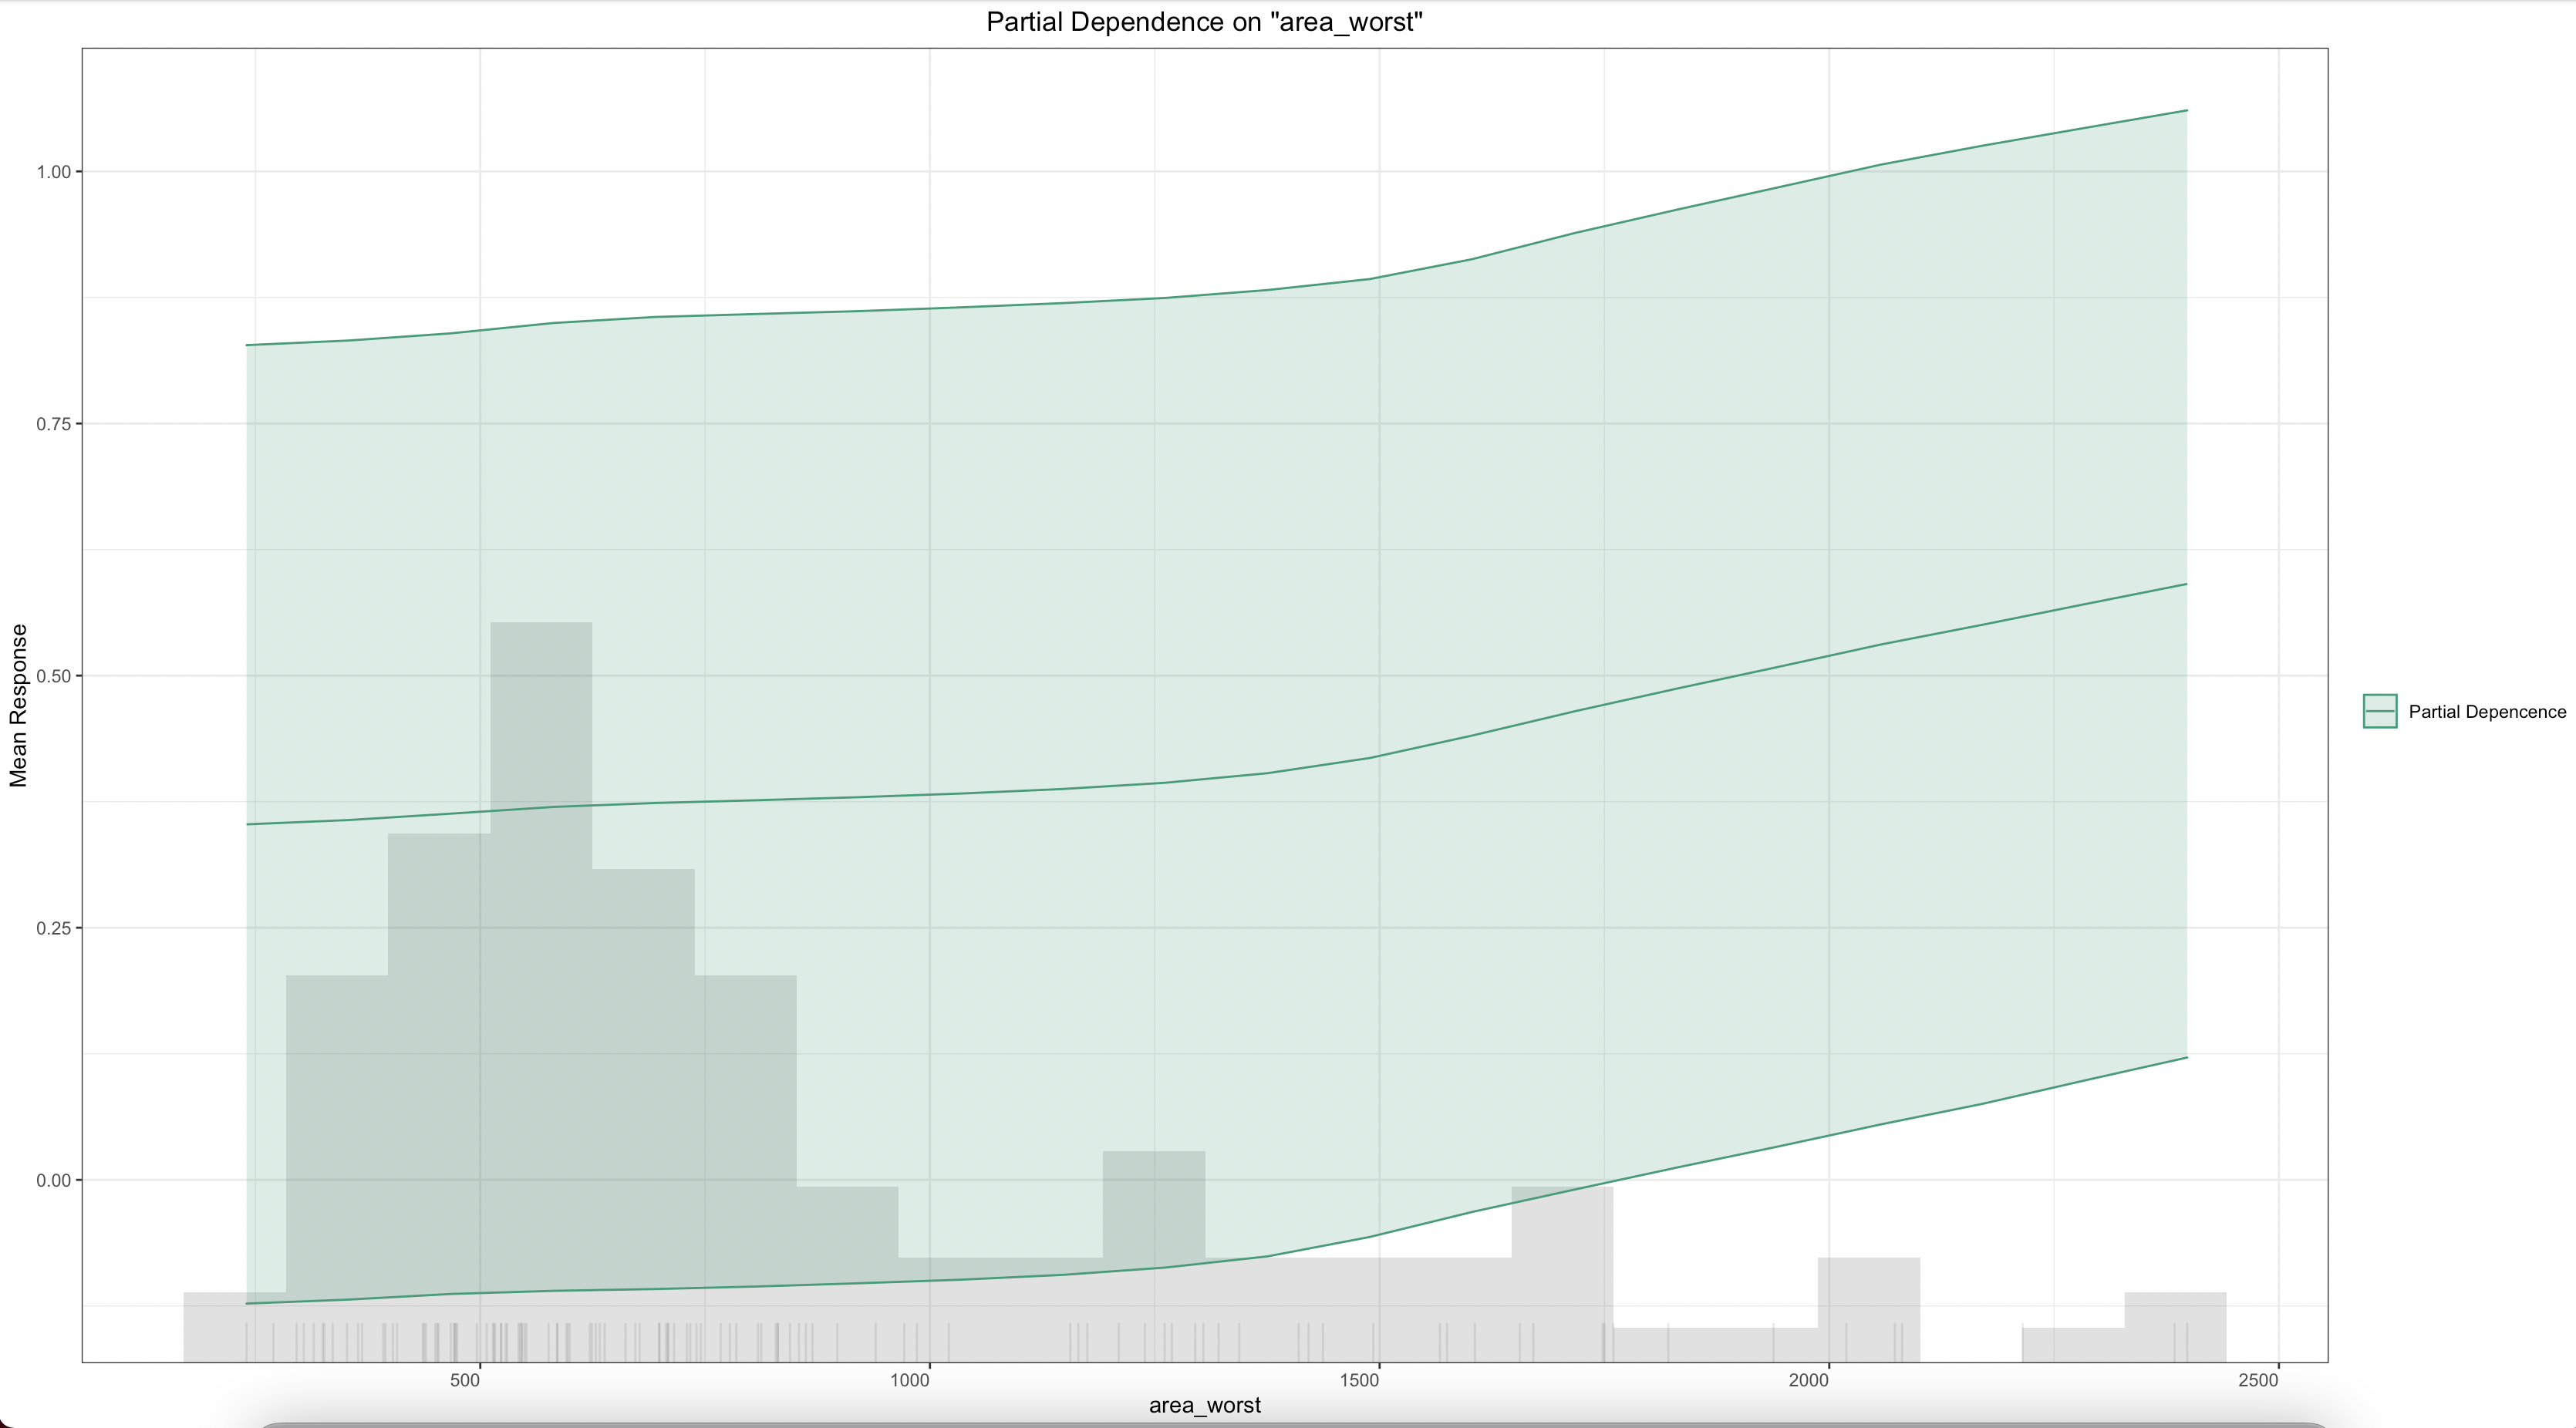
\includegraphics[width=0.8\textwidth]{images/pd_plot.png}
    \caption{Partial Dependence Plot wrt area\_worts}
    \label{fig:pd_plot}
\end{figure}

\begin{figure}
    \centering
    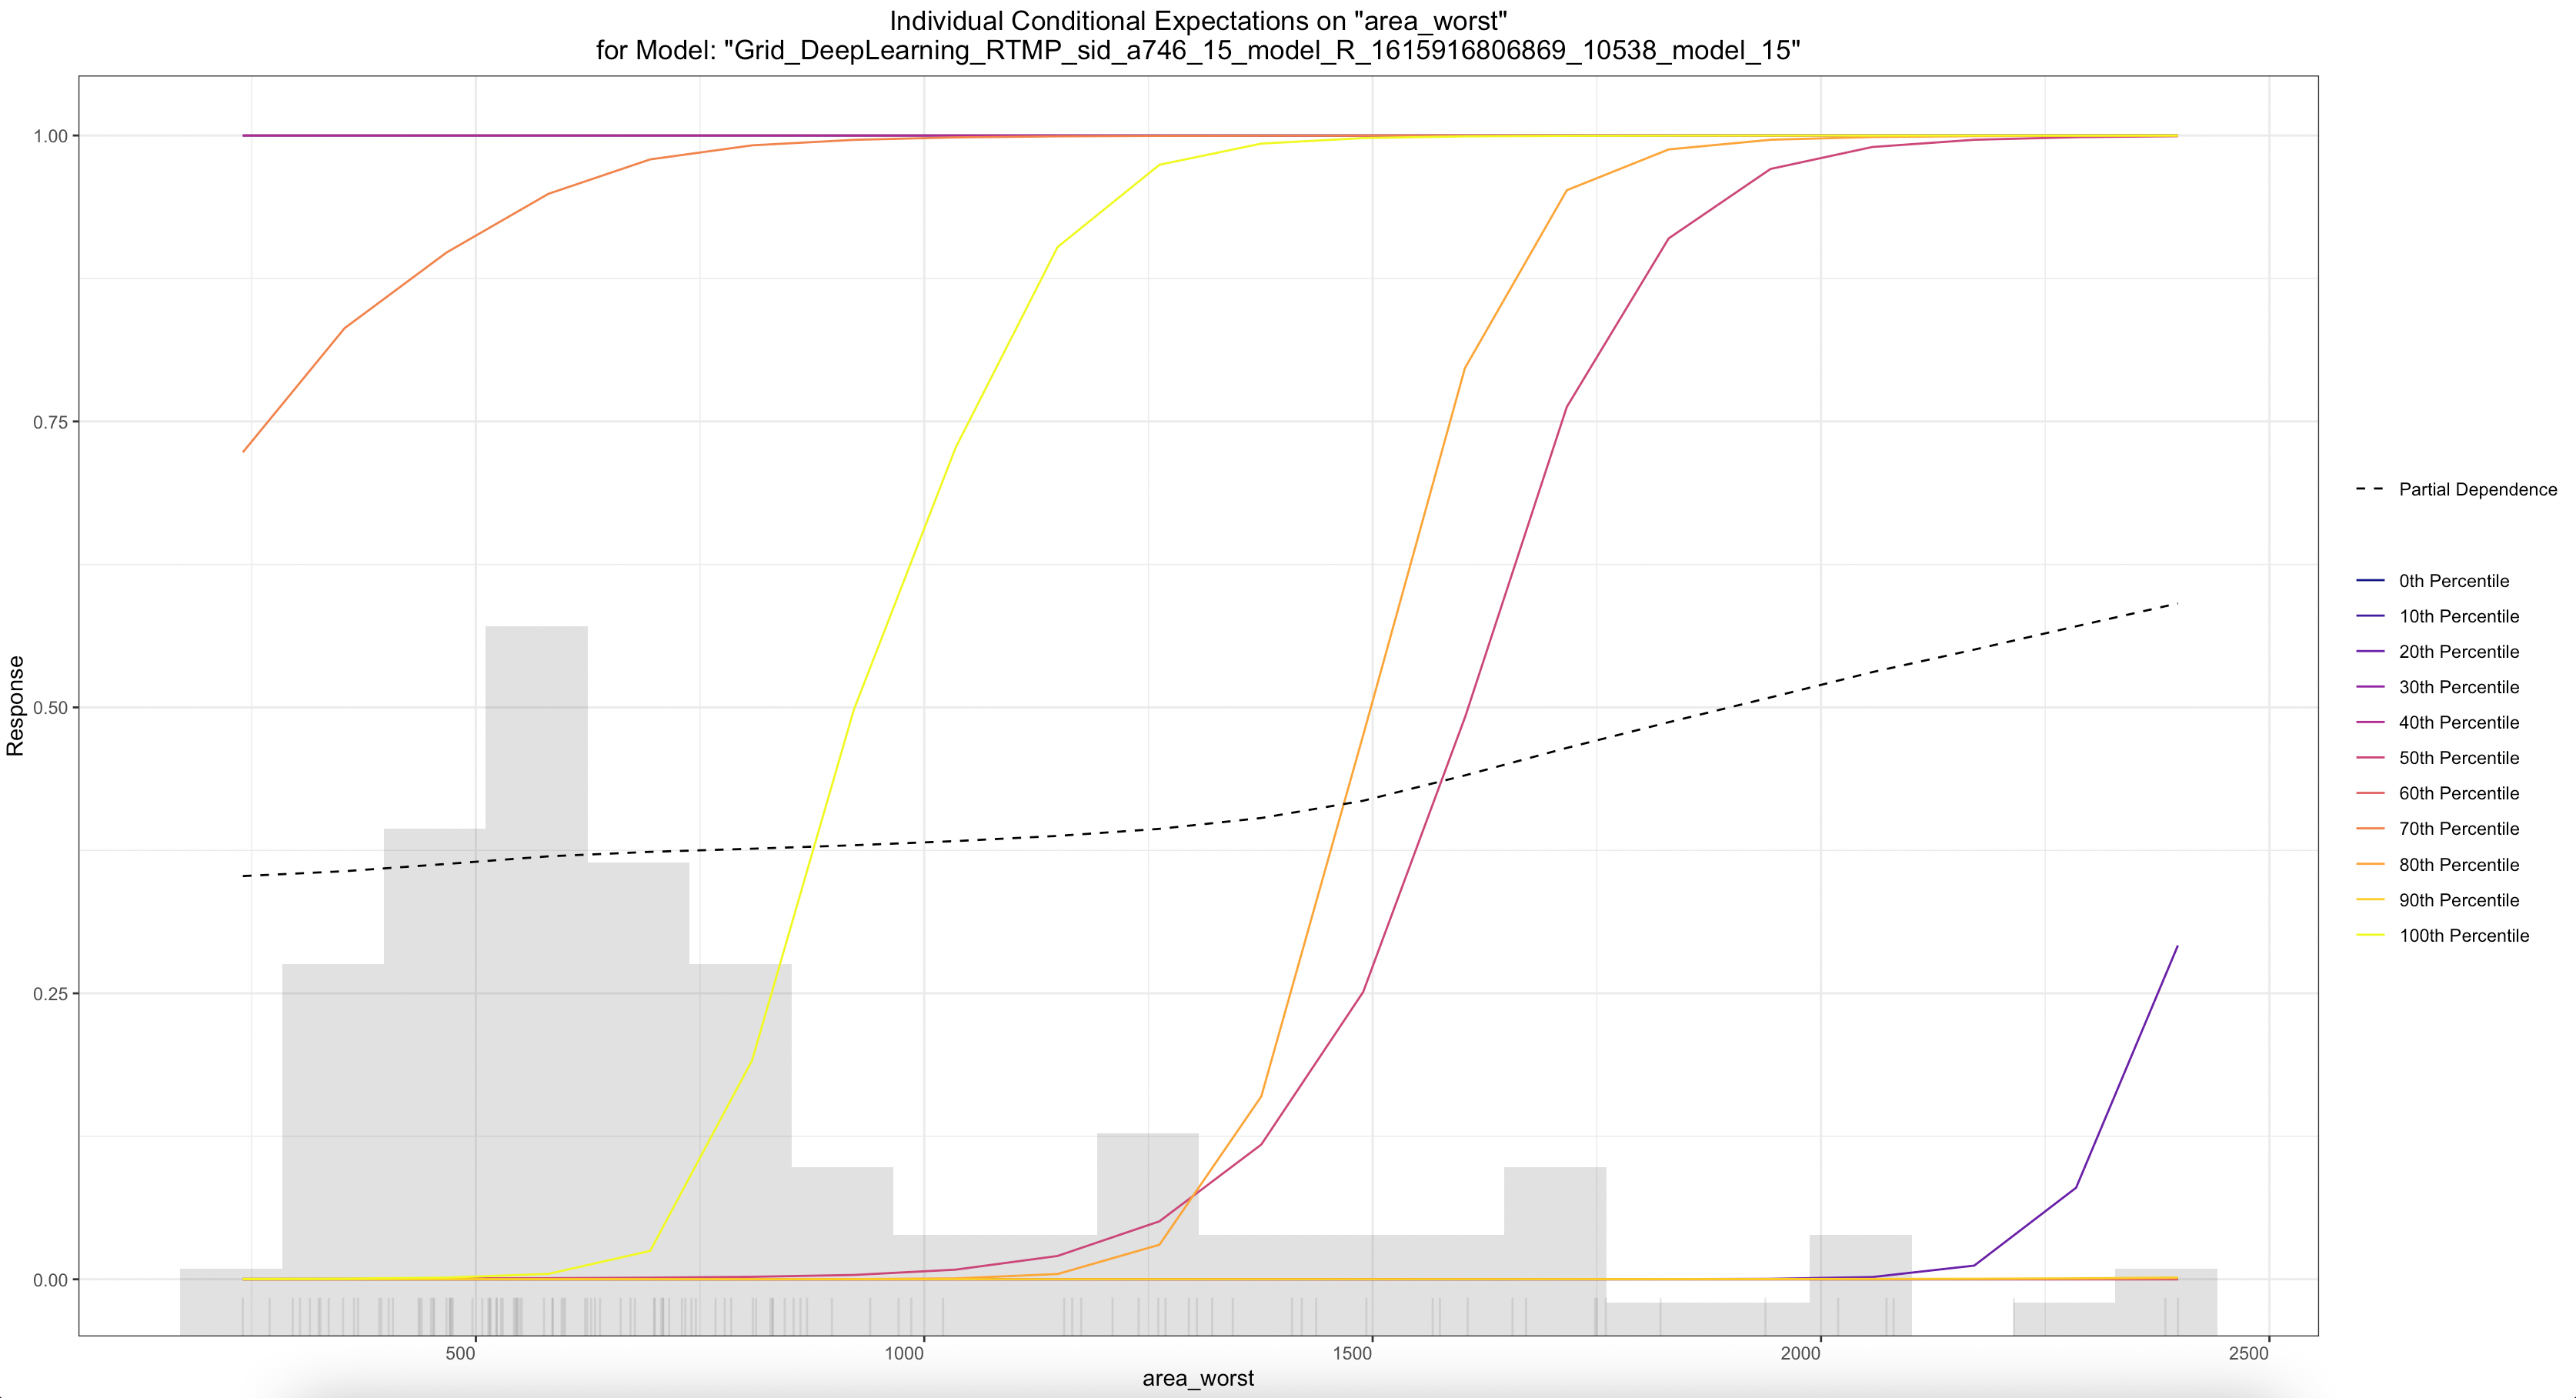
\includegraphics[width=0.8\textwidth]{images/ice_plot.png}
    \caption{Conditional Expectation Plot wrt area\_worst}
    \label{fig:ice_plot}
\end{figure}

\section{Final Assessment}\label{final-assessment}

We compare the logistic regression and the neural networks wrt accuracy
and sensitivity and specificity on the test set.

\begin{center}
 \begin{tabular}{|c | c |  c | c|} 
 \hline
 Model & Accuracy & Sensitivity/Recall & Specificity \\ [0.5ex] 
 \hline
 \hline
 Logistic regression & .965 & .929 & .986 \\ 
 \hline
 Neural Network & .982 & .976 &  .986 \\
 \hline
\end{tabular}
\end{center}

The neural network performs better in accuracy with only 2
misclassifications on the test set whereas the logistic regression
misclassifies in 4 cases. The difference in errors is due to the better
sensitivity of the neural network: only 1 malignant tumor was wrongly
classified, whereas the logistic regression did err in 3 cases.

\begin{figure}
    \centering
    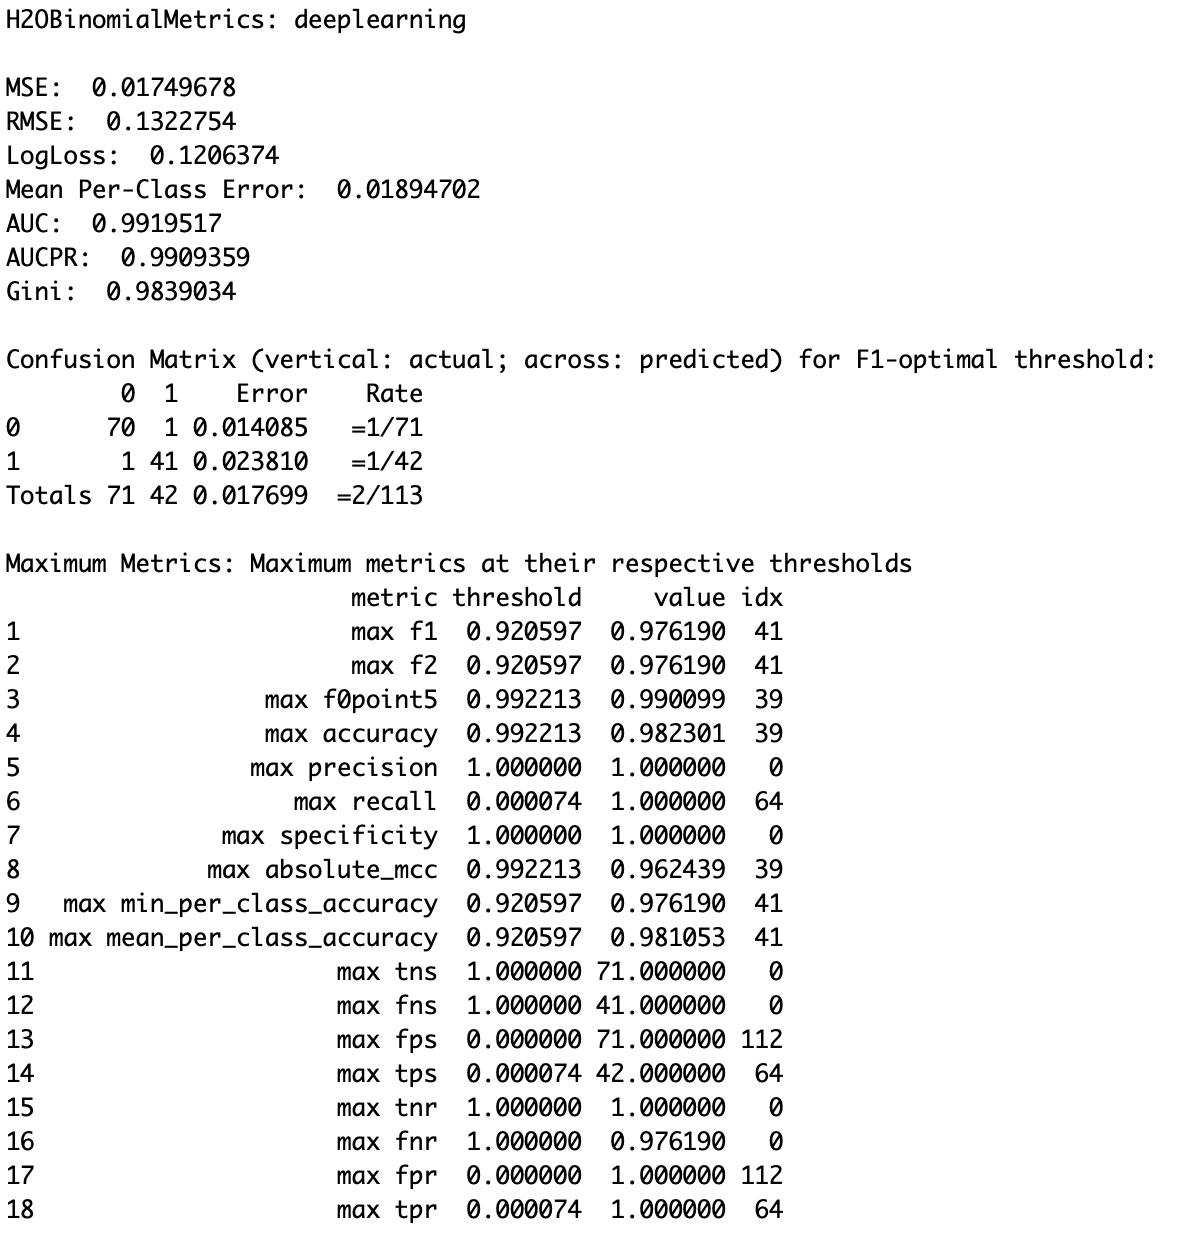
\includegraphics[width=0.8\textwidth]{images/h2o_model_performance.png}
    \caption{Metrices of the choosen Artificial Neural Network}
    \label{fig:h2o_model_performance}
\end{figure}

please, see the notebooks (of specific model) for more details.

\section{Future Work}\label{future-work}

Interpretation and explainability are important topics in machine
learning and a fundamental requirement in the medical domain. We would
like to, on one hand improve accuracy and especially sensitivity of the
neural network model we have build. On the other hand, we would like to
investigate (and improve) the connection between the logistic regression
and the neural network and use the logistic regression to obtain
interpretation and explanations. If we can find and point out
connections of logistic regression and neural network interpretation and
explanation from logistic regression can be meaningful for the neural
network, too.

Shifting the focus in logistic regression from performance to
interpretability we would drop the PCA preprocessing. Insted of feature
reduction by PCA we would start with the features the neural network
output as important variables.

Why we think there is a connection between logistic regression and
neural networks: A neural network with sigmoid activation is basically a
collection of logistic regression models: Every node in the first hidden
layer is a logistic regression. Would we connect the hidden layer node
with the suitable loss function we would obtain a classification
algorithm. The neural network can be more powerful since it uses several
nodes in its (first) hidden layeer. Additional power requires these
individual regressions to act differently and to be combined in a
meaningful way (if all logistic regressions did the same, there would be
no improvement). This task has to be solved by the network, through
optimization with respect to the final classification. We would like to
further investigate this.

Interpretation and explanations for logistic regression are already
available. We would start applying them to our task.

\renewcommand\refname{References}
\bibliography{references.bib}

\end{document}
